\documentclass[../main.tex]{subfiles}
 

\begin{document}

\chapter{Program Structure}\label{sec: ProgramStructure}


\section{Variational Monte Carlo Simulations}

The variational Monte Carlo (VMC) code consists primarily of several classes. A quick overview of these classes is available in Appendix \ref{sec: Program Structure Appendix}. The \textbf{Particle} class stores information about a single particles position, and is responsible for changing this position when necessary and providing it to other parts of the program. The \textbf{System} class contains information about the system, such what kind of Hamiltonian and wave function we have. It also has a vector containing instances of the \textbf{Particle} class, one instance for each particle in the system. In addition this class is responsible for running the Metropolis algorithm, including checking if the Metropolis step is accepted, and calculating the drift (quantum) force and Greens function when using importance sampling. The \textbf{Sampler} class is responsible for sampling the energy etc. after each step and computing averages at the end of the simulation.

The \textbf{Hamiltonian} class is responsible for calculating the Hamiltonian, i.e. the kinetic part, the non-interacting potential part, and also the interacting potential part if interactions are included. In addition, the \textbf{Hamiltonian} class contains the functions for calculating the single-particle wave functions and its gradient and Laplacian. The last part was initially done in the \textbf{WaveFunction} class, but when including different types of potentials it turned out to be more convenient to evaluate the single-particle wave functions etc. in the \textbf{Hamiltonian} class. The \textbf{WaveFunction} class deals with the more general things concerning the many-body wave function, such as updating the Slater determinant and evaluating the full many-body wave function and its gradient and Laplacian. It receives the single-particle wave function evaluations from the \textbf{Hamiltonian} class when they are needed. The \textbf{WaveFunction} class also contains the function for calculating the Metropolis ratio, which the \textbf{System} class uses to determine if a given step is accepted or not. 

The \textbf{InitialStates} class sets up an initial state for the particles, i.e. it creates instances of the \textbf{Particle} class and gives them their initial positions. The \textbf{VariationMethods} class contains methods for variation of the variational parameters. Currently the only method implemented is the steepest descent method, however the program is set up in a way which makes adding other methods, such as the more advanced conjugate gradient method, fairly simple.

\subsection{Initializing}

The program starts in the "main.cpp" file where system settings such as number of dimensions, number of particles and number of Monte Carlo cycles, and also constants such as the harmonic oscillator frequency $\omega$ are defined. Certain flags are also set to true or false, such as whether to include interactions or not, and what type of potential is used. 

An instance of the \textbf{InitialStates} class is then created which sets up initial positions for each particle where, for each dimension, the particle is given a random value uniformly distributed between $0$ and $1$ as its position in that dimension. For each particle, an instance of the \textbf{Particle} class is created, which is given the position for that particle. In addition, every other particle has its positions in each dimension multiplied by $-1$. This is done so that when we have a double well with a barrier between the wells at e.g. $x=0$, the total amount of particles will be evenly split between the wells. The seed used to generate random positions is dependent on the "m\_my\_rank" variable, which is decided by which node we are on when running the program in parallel. This is because we need to give the nodes different initial states from each other, to avoid running the exact same simulation on every node. 

\lstset{language=c++}
\begin{lstlisting}[title={Setting up the Initial State}]
void RandomUniform::setupInitialState() {

    long idum = -1-m_my_rank;
    Random::setSeed(idum);

    // Create random positions for all particles:
    for (int i=0; i < m_numberOfParticles; i++) {
        std::vector<double> position = std::vector<double>();

        for (int j=0; j < m_numberOfDimensions; j++) {
            double pos = pow(-1, i%2)*Random::nextDouble();
            position.push_back(pos);
        }
        // Create particles:
        m_particles.push_back(new Particle());
        m_particles.at(i)->setNumberOfDimensions(m_numberOfDimensions);
        m_particles.at(i)->setPosition(position);
    }
}
\end{lstlisting}

Next, in "main.cpp", an instance of the \textbf{Hamiltonian} class is created as well as an instance of the \textbf{WaveFunction} class. All three instances are then stored in an instance of the \textbf{System} class, which proceeds to run the Metropolis algorithm.



\subsection{Monte Carlo}

The \textbf{System} class is responsible for running the Metropolis algorithm. It loops over the number of Metropolis steps and the number of particles and changes the position of the particle. The change in position depends on whether or not we use importance sampling (the Metropolis-Hastings algorithm). If we do not use importance sampling the change in position is chosen by a random uniform distribution independent of the state of the system. Based on the change in position the \textbf{WaveFunction} class calculates the Metropolis ratio, which is used to determine if the position change is accepted or not. If importance sampling is used the change in position depends on the so-called quantum force, and the Metropolis ratio is also dependent on the Greens function which in turn depends on the quantum force. Both the quantum force and the Greens function are calculated in the \textbf{System} class. 

The ratio used to determine whether or not to accept the step is compared to a random uniformly distributed number between $0$ and $1$. A ratio greater or equal to the random number results the step being accepted. If the position change is accepted it is kept, otherwise it is reverted, and then the entire system with its current particle positions is sampled by the \textbf{Sampler} class. 

The \textbf{Sampler} class adds the energy of the system at each step to the cumulative energy, and computes the average after the loop over Metropolis steps has finished. However, not every Metropolis step is sampled. Before we start sampling we let the system run through some steps (e.g. $10\%$ of the total amount) in order to let the system equilibrate first. Below is the code for handling a Metropolis step when we are not using importance sampling. The change in position is first applied to the particle in the "computeMetropolisRatio" function of the \textbf{WaveFunction} class, and then reverted in this listed function if the step is not accepted.

\lstset{language=c++}
\begin{lstlisting}[caption={Metropolis Step Without Importance Sampling}]
bool System::metropolisStep(int currentParticle) {
    /* Perform the actual Metropolis step: Take the current particle and
     * change its position by a random amount, and check if the step is
     * accepted by the Metropolis test (compare the wave function evaluated
     * at this new position with the one at the old position).
     */

    // Change position of current particle by a random amount creating a trial state
    setCurrentParticle(currentParticle);
    std::vector<double> positionChange(m_numberOfDimensions);

    for (int i=0; i<m_numberOfDimensions; i++){
        positionChange[i] = (Random::nextDouble()*2-1)*m_stepLength;
    }

    // Metropolis ratio
    double qratio = m_waveFunction->computeMetropolisRatio(m_particles, currentParticle, positionChange);

    // Check if trial state is accepted
    if (Random::nextDouble() <= qratio){
        m_waveFunction->updateSlaterDet(currentParticle);
        return true;
    }

    for (int i=0; i<m_numberOfDimensions; i++){
        // If trial state is not accepted, revert to old position for chosen particle (revert to old state)
        m_particles[currentParticle]->adjustPosition(-positionChange[i], i);
        m_waveFunction->updateDistances(currentParticle);
        m_waveFunction->updateSPWFMat(currentParticle);
        m_waveFunction->updateJastrow(currentParticle);
    }

    return false;
}
\end{lstlisting}


\subsection{Virtual Functions}

Virtual functions are an essential part of how the \textbf{Hamiltonian} and \textbf{WaveFunction} classes are built up. Normally if a super class has defined a function and a sub class defines an identical function, the super class function overwrites the sub class function. However, if we make the super class function virtual, the sub class function will not be overwritten by the compiler. This is useful because it allows us to have a super class with multiple sub classes where each sub class has its own implementation of a given function which is virtual in the super class. For example, our \textbf{Hamiltonian} class has sub classes for different types of Hamiltonians (i.e. HO well, double HO well, square well, etc.). Depending on the system we are looking at, we create an instance of the sub class corresponding to the Hamiltonian of the system. By doing this we can do a general call to a function which all sub classes of the \textbf{Hamiltonian} class have, but have implemented in different ways. The implementation that is used will then be the one belonging to the sub class we created the instance of. 

Let us look at a more concrete example to make it more clear. Each sub class of the \textbf{Hamiltonian} class has an implementation of the "computeLocalEnergy" function. The difference between the function implementation for the double HO well and the regular HO well is how the potential energy is calculated.

\lstset{language=c++}
\begin{lstlisting}[label={lst:Regular Well Potential}, caption={Potential energy calculation for the regular harmonic oscillator well sub class of the \textbf{Hamiltonian} class.}]
double potentialEnergy = 0;
    double repulsiveTerm = 0;

    for (int i=0; i < numberOfParticles; i++){
        double rSquared = 0;
        std::vector<double> r_i = particles[i]->getPosition();
        for (int k=0; k < numberOfDimensions; k++){
            rSquared += r_i[k]*r_i[k];
        }
        potentialEnergy += rSquared;

        for (int j=i+1; j < numberOfParticles; j++){
            double r_ijSquared = 0;
            std::vector<double> r_j = particles[j]->getPosition();
            for (int k=0; k < numberOfDimensions; k++){
                    r_ijSquared += (r_i[k] - r_j[k]) * (r_i[k] - r_j[k]);
            }

            double r_ij = sqrt(r_ijSquared);
            repulsiveTerm += 1./r_ij;
        }
    }
    potentialEnergy *= 0.5*m_omega*m_omega;
    if (m_repulsion) { potentialEnergy += repulsiveTerm; }
\end{lstlisting}

\lstset{language=c++}
\begin{lstlisting}[label={lst:Double Well Potential}, caption={Potential energy calculation for the double harmonic oscillator well sub class of the Hamiltonian class.}]
double potentialEnergy = 0;
    double repulsiveTerm = 0;

    for (int i=0; i < numberOfParticles; i++){
        double rSquared = 0;
        double term2 = 0;
        double term3 = 0;

        std::vector<double> r_i = particles[i]->getPosition();
        for (int k=0; k < numberOfDimensions; k++){
            rSquared += r_i[k]*r_i[k];
            term2 += 2.*abs(r_i[k])*m_L(k);
            term3 += m_L(k)*m_L(k);
        }

        potentialEnergy += rSquared - term2 + term3;

        for (int j=i+1; j < numberOfParticles; j++){
            double r_ijSquared = 0;
            std::vector<double> r_j = particles[j]->getPosition();
            for (int k=0; k < numberOfDimensions; k++){
                    r_ijSquared += (r_i[k] - r_j[k]) * (r_i[k] - r_j[k]);
            }

            double r_ij = sqrt(r_ijSquared);
            repulsiveTerm += 1./r_ij;
        }
    }

    potentialEnergy *= 0.5*m_omega*m_omega;

    if (m_repulsion) { potentialEnergy += repulsiveTerm; }
\end{lstlisting}

At the start of the program we can use one of the following lines of code to choose which of the two Hamiltonians we are using for the simulation. (We can of course choose any other implemented Hamiltonian sub class as well.)
\lstset{language=c++}
\begin{lstlisting}[caption={Setting the Hamiltonian of the system.}, label={lst:Choose Hamiltonian}]
system->setHamiltonian      (new HarmonicOscillatorElectrons(system, omega, analyticalKinetic, repulsion));
system->setHamiltonian      (new DoubleHarmonicOscillator(system, L, omega, analyticalKinetic, repulsion));
\end{lstlisting}
This will store the instance we chose in the "m\_hamiltonian" object of the \textbf{System} class. Now we can call the "computeLocalEnergy" function from the \textbf{Sampler} class with the following line.
\lstset{language=c++}
\begin{lstlisting}[caption={Calling the "computeLocalEnergy" function from the \textbf{Sampler} class. The function implementation used will be the one belonging to the \textbf{Hamiltonian} sub class we have chosen as the Hamiltonian of the system.}]
std::vector<double> energies = m_system->getHamiltonian()->computeLocalEnergy(m_system->getParticles());
\end{lstlisting}
Here the "m\_system->getHamiltonian()" call returns the "m\_hamiltonian" object, and the "m\_system->getParticles()" call returns the "m\_particles" vector which is used as argument for the "computeLocalEnergy" function, so the call is essentially 
\begin{lstlisting}
m_hamiltonian->computeLocalEnergy(m_particles);
\end{lstlisting}
The program will then call the implementation of the "computeLocalEnergy" function which corresponds to the sub class instance we have stored in "m\_hamiltonian". If we chose line $1$ in Listing \ref{lst:Choose Hamiltonian}, then the code in Listing \ref{lst:Regular Well Potential} will be used, while if we chose line $2$, then the code in Listing \ref{lst:Double Well Potential} will be used. This saves us from having to use an if-test every time we want to call the "computeLocalEnergy" function. Instead we just need one if-test at the beginning to choose between line $1$ and $2$ in Listing \ref{lst:Choose Hamiltonian}. This is significant for optimizing the program when we might have millions of Monte Carlo cycles, since we avoid millions of if-tests, and it also makes the code a lot cleaner. Using virtual functions in this way is a form of polymorphism, which is the concept of "providing a single interface to entities of different types."\textsuperscript{\cite{Stroustrup}}

There are two types of virtual functions we can use in C++; the regular virtual functions and pure virtual functions. When a virtual function is defined in a super class, the compiler requires that function to always have a valid implementation. This means that if the super class only defines the function, but does not provide a proper implementation of the function, then every sub class of the super class has to provide an implementation. This is what is called a pure virtual function. The alternative is a regular virtual function, which is a function which is defined as virtual in the super class, but also has an implementation in the super class. 

The implementation in the super class then acts as a default implementation, which will be used if the instanced sub class does not have its own implementation of said function. If the sub class does have its own implementation this will be used instead of the default. This can be useful if some of the sub classes have the same implementation of a given function while other sub classes have unique implementations. The sub classes who share an implementation can use the default implemented by the super class, while the other sub classes can use their own unique implementations. This way we do not have to implement the exact same function several times, and the amount of code is reduced. Another use for the default implementation is if some sub classes have unique implementations of a given function, but other sub classes do not need to have the function at all. If a pure virtual function was used, then every sub class that did not need the function would still need a dummy version of the function. This dummy version would not do anything and would never be called, but would still be necessary for compiling the program. Instead we can use a regular virtual function, where the default version implemented in the super class is a dummy version, which then allows the sub classes that do not need the function to skip implementing it.

\lstset{language=c++}
\begin{lstlisting}[caption={Example of definitions of a pure virtual function (line $1$) and a regular virtual function with a dummy implementation (line $2$).}]
virtual std::vector<double> computeLocalEnergy(std::vector<class Particle*> particles) = 0;
virtual std::vector<double> computeLocalEnergy(std::vector<class Particle*> particles) { particles = particles; }
\end{lstlisting}

The pure virtual functions can also be useful. For example, if you know that every sub class should have its own unique implementation of a function, then the lack of a default implementation can act as a test or safeguard for the code when implementing new sub classes. If you forget to implement the function, the compiler will abort and give an error. You will then be made aware that something is wrong, instead of potential using a (wrong) default implementation, which makes it seem like the program is running fine, while it is actually providing erroneous results. The "computeLocalEnergy" function in the VMC program is an example of a pure virtual function, so if someone wanted to add a new Hamiltonian to the program they would have to implement this function for the new Hamiltonian.

\subsection{Hamiltonians}\label{sec:Hamiltonians}

The main job for the \textbf{Hamiltonian} class is to compute the local energy. This means that it has to calculate the energy from the external potential (e.g. harmonic oscillator well), the kinetic energy of the particles, and, if included, the potential energy from particle-particle interactions (e.g. Coulomb repulsion). In this thesis we look at electrons in different types of external potentials, and therefore we have Coulomb repulsion as the particle-particle interaction. The kinetic energy can be computed with numerical differentiation or using analytical expressions for the Laplacian of the wave function. The numerical differentiation can be implemented generally for any Hamiltonian, so we can implement a function for it once, in the \textbf{Hamiltonian} super class, and then call it from the sub class we are using. This is done by the following function.
\lstset{language=c++}
\begin{lstlisting}[caption={Function for calculating the kinetic energy by numerical differentiation. The function is general for all the sub classes of the \textbf{Hamiltonian} class, and is therefore implemented once, in the super class "hamiltonian.cpp".}]
double Hamiltonian::computeKineticEnergy(std::vector<Particle*> particles){
    // Compute the kinetic energy using numerical differentiation.
    double numberOfParticles = m_system->getNumberOfParticles();
    double numberOfDimensions = m_system->getNumberOfDimensions();
    double h = 1e-4;

    // Evaluate wave function at current step
    double waveFunctionCurrent = m_system->getWaveFunction()->evaluate(particles);
    double kineticEnergy = 0;

    for (int i=0; i < numberOfParticles; i++){
        for (int j=0; j < numberOfDimensions; j++){
        
            // Evaluate wave function at forward step
            particles[i]->adjustPosition(h, j);
            m_system->getWaveFunction()->updateDistances(i);
            m_system->getWaveFunction()->updateSPWFMat(i);
            m_system->getWaveFunction()->updateJastrow(i);
            double waveFunctionPlus = m_system->getWaveFunction()->evaluate(particles);

            // Evaluate wave function at backward step
            particles[i]->adjustPosition(-2*h, j);
            m_system->getWaveFunction()->updateDistances(i);
            m_system->getWaveFunction()->updateSPWFMat(i);
            m_system->getWaveFunction()->updateJastrow(i);
            double waveFunctionMinus = m_system->getWaveFunction()->evaluate(particles);

            // Part of numerical diff
            kineticEnergy -= (waveFunctionPlus - 2*waveFunctionCurrent + waveFunctionMinus);

            // Move particles back to original position
            particles[i]->adjustPosition(h, j);
            m_system->getWaveFunction()->updateDistances(i);
            m_system->getWaveFunction()->updateSPWFMat(i);
            m_system->getWaveFunction()->updateJastrow(i);
        }
    }
    // Other part of numerical diff. Also divide by evaluation of current wave function and multiply by 0.5 to get the actual kinetic energy.
    kineticEnergy = 0.5*kineticEnergy / (waveFunctionCurrent*h*h);
    return kineticEnergy;
}
\end{lstlisting}

If we use analytical expressions for the Laplacian when calculating the kinetic energy, then we call the "computeDoubleDerivative" function from the \textbf{WaveFunction} class. When calculating the local energy, the difference from sub class to sub class will be the calculation of the external potential energy as shown in Listing \ref{lst:Regular Well Potential} and Listing \ref{lst:Double Well Potential}. In addition to calculating the local energy, the \textbf{Hamiltonian} sub classes also contain functions for evaluating the single particle wave function and its gradient and Laplacian. Since the single particle wave functions contain Hermite polynomials we also calculate these in the \textbf{Hamiltonian} sub classes. The Hermite polynomials are analytical expressions, but they also have a recursive relation. Therefore we can either implement them by writing out the analytical expression for every Hermite polynomial we might need and then choose the one we need at a given moment, or we can calculate them recursively. There are advantages to each of these implementations. The recursive method requires less code and is therefore quicker to implement and is general, so that it will work regardless of how many particles we put in the system. However, since it needs to iterate from the lowest polynomial every time, it can become very computationally expensive when we have a lot of particles. 

Using the analytical expressions we would have to add enough polynomials to support the amount of particles we want in the system, and if we wanted to increase the number of particles further, we would have to implement more analytical expressions. There are two ways we could use for choosing among the analytical expressions. The simplest is to just have an if-test for every expression and then start at the beginning and check if we wanted to use $H_0$ (the lowest Hermite polynomial). If not we would move on to the if-test for $H_1$ and then continue like that until we found the one we wanted to use and return that. This might be computationally faster than the recursive method, but it would still potentially need to go through a lot of if-tests, especially when the number of particles in the system is high. There is a more optimized alternative, but it is more difficult to implement. Instead of of using if-tests to check every expression from the start until we find the one we want, we can instead store all the expressions in a list, and then use the index for the expression we want to get it from the list without having to touch any of the other expressions at all. In this thesis the recursive method was used originally, however a switch to the last method described was made eventually, which is further discussed in section \ref{sec:Optimizing Hermite}.

\lstset{language=c++}
\begin{lstlisting}[caption={Recursive method for computing Hermite polynomials. This method requires the least amount of code and will work for any amount of particles in the system. However, it is also the least optimized method in terms of computation time, and it can be very time consuming when the amount of particles is high.}]
double HarmonicOscillatorElectrons::computeHermitePolynomial(int nValue, double position) {
    // Computes Hermite polynomials.
    double alphaSqrt = sqrt(m_alpha);
    double omegaSqrt = sqrt(m_omega);
    double factor = 2*alphaSqrt*omegaSqrt*position;

    double HermitePolynomialPP = 0;                 // H_{n-2}
    double HermitePolynomialP = 1;                  // H_{n-1}
    double HermitePolynomial = HermitePolynomialP;  // H_n

    for (int n=1; n <= nValue; n++) {
        HermitePolynomial = factor*HermitePolynomialP - 2*(n-1)*HermitePolynomialPP;
        HermitePolynomialPP = HermitePolynomialP;
        HermitePolynomialP = HermitePolynomial;
    }

    return HermitePolynomial;
}
\end{lstlisting}

\subsection{Wave Functions}

The \textbf{WaveFunction} class is responsible for maintaining and evaluating the full wave function of the system. The systems we are looking at in this thesis are systems where a chosen number of electrons are confined in various external potentials. The wave function then approximated by a Slater determinant of the single particle wave functions, and a Jastrow factor (if interactions are included). Since the single particle functions are implemented in the Hamiltonian sub classes as discussed above, we do not need different sub classes of the \textbf{WaveFunction} class for different external potentials. Two sub classes of the \textbf{WaveFunction} class are used here; The \textbf{ManyElectrons} sub class and the \textbf{ManyElectronsCoefficients} sub class. The first one is used for regular variational Monte Carlo simulations of the systems we are looking at, while the second uses diagonalization of a general potential well to expand its solutions in terms of harmonic oscillator functions. For the most part these two sub classes have the implementation, with the difference between them being how the single particle wave functions in the Slater matrix are approximated.

Before the Monte Carlo simulation starts, the \textbf{WaveFunction} sub classes set up several matrices. The "setUpSlaterDet" function sets up the Slater matrix of single particle wave functions, and matrices for its gradient and Laplacian. We split the Slater matrix in one spin up part and one spin down part, both of which are square matrices. However, even though we treat them as two different matrices we store them together in the matrix called "m\_SPWFMat". The first half of the particles are considered spin up, while the other half are considered spin down. We also store the inverse of the spin up part and the spin down part separately in their own matrices. The "setUpDistances" function sets up a matrix containing the distances between particle pairs, i.e. element $ij$ is the distance between particle $i$ and particle $j$. The "setUpJastrowMat" function sets up matrices for the Jastrow factor and its gradient. The latter two functions are used to optimize performance and will be discussed more later. The sub classes of the \textbf{WaveFunction} class also contains functions for updating the matrices at every Metropolis step. 

The "evaluate" function evaluates the total wave function which is used when computing the kinetic energy using numerical differentiation in the Hamiltonian class. Since we split the Slater determinant into a spin up part and a spin down part, we need to implement a special case for when we only have one particle in the system. Since the one particle can not have both spin up and spin down, one of the Slater matrices will be empty, and since we use the product of the spin up determinant and the spin down determinant normally, we have to choose one of them and exclude the other. Here we have chosen to give the single particle spin up in the one particle case.

\lstset{language=c++}
\begin{lstlisting}
double ManyElectrons::evaluate(std::vector<class Particle*> particles) {
    // Evaluates the wave function using brute force.

    mat spinUpSlater;
    mat spinDownSlater;
    if (m_numberOfParticles == 1) {
        spinUpSlater = zeros<mat>(m_numberOfParticles, m_numberOfParticles);
        spinDownSlater = zeros<mat>(m_numberOfParticles, m_numberOfParticles);
        spinUpSlater(0,0) = m_SPWFMat(0,0);
    }
    else {
        spinUpSlater = zeros<mat>(m_halfNumberOfParticles, m_halfNumberOfParticles);
        spinDownSlater = zeros<mat>(m_halfNumberOfParticles, m_halfNumberOfParticles);

        for (int i=0; i < m_halfNumberOfParticles; i++) {
            for (int j=0; j < m_halfNumberOfParticles; j++) {
                spinUpSlater(i,j) = m_SPWFMat(i,j);
                spinDownSlater(i,j) = m_SPWFMat(i+m_halfNumberOfParticles,j);
            }
        }
    }

    double beta = m_parameters[1];
    double exponent = 0;
    if (m_Jastrow) {
        for (int i=0; i < m_numberOfParticles; i++) {
            for (int j=i+1; j < m_numberOfParticles; j++) {
                exponent += m_JastrowMat(i,j);
            }
        }
    }

    double waveFunction;
    if (m_numberOfParticles == 1) {
        waveFunction = det(spinUpSlater)*exp(exponent);
    }
    else {
        waveFunction = det(spinDownSlater)*det(spinUpSlater)*exp(exponent);
    }

    return waveFunction;
}
\end{lstlisting}
Similarly, there are functions for evaluating the gradient and Laplacian of the full wave function. The gradient  for the Slater part and Jastrow (correlation) part of the wave function are computed separately and then combined afterwards, which is also the case for the Laplacian. The full gradient is simply the two parts added together, but for the Laplacian we get an additional cross term equal to two times the gradient parts multiplied together. This is shown in Eq.~(\ref{eq: TotalLaplacian}). There is also a function for calculating the derivative of the wave function with respect to the variational parameters, which is needed when doing the variation of parameters.

The Metropolis ratio is also calculated in the sub classes of the \textbf{WaveFunction} class, and in our case, since the full wave function is made up of a Slater determinant and a Jastrow factor, we can write the Metropolis ratio as a product of a Slater part and a Jastrow part. From Eq.~(\ref{eq:MetropolisRatioSD}) we know that the expression for the Slater part of the ratio is
\begin{align}
    R_{SD} = \sum_{j=1}^N \phi_j({\bf r}_i^{\textrm{new}}) d_{ji}^{-1}({\bf r}^{\textrm{old}}),
\end{align}
where $\phi$ are the single particle wave functions, and $d_{ji}^{-1}$ is element $ji$ of the inverse Slater matrix. From Eq.~(\ref{eq:MetropolisRatioC}) we know the expression for the Jastrow part
\begin{align}
    R_{C} = \exp\left(\sum_{i=1, i\neq k}^{N} f_{ik}^{\textrm{new}} - f_{ik}^{\textrm{old}}\right),
\end{align}
where $N$ is the number of particles and
\begin{align}
    f_{ij} = \frac{a r_{ij}}{(1+\beta r_{ij})}.
\end{align}
In the code we tabulate the necessary values in matrices that are maintained in other functions, which makes the code for the Metropolis ratio very clean with just a few simple loops.
\lstset{language=c++}
\begin{lstlisting}[caption={The computation of the Metropolis ratio when the full wave function consists of a Slater determinant and a Jastrow factor. The ratio can be split into a Slater part and a Jastrow part which are multiplied together to form the full ratio. The "m\_spinUpSlaterInverse" matrix is the inverse of the spin up Slater matrix, and similarly for the spin down matrix, while "m\_SPWFMat" is a matrix containing the single particle wave functions, i.e. it is the spin up and spin down Slater matrices stored together in one matrix. The "m\_JastrowMat" matrix contains the exponent of the Jastrow factor for all particle pairs for the trial state, while the "m\_JastrowMat" is the same matrix, but for the last accepted state (i.e. the state before the trial state).}]
int i = currentParticle;
double ratioSlaterDet = 0;
if (i < m_halfNumberOfParticles) {
    for (int j=0; j < m_halfNumberOfParticles; j++) {
        ratioSlaterDet += m_spinUpSlaterInverse(j,i)*m_SPWFMat(i,j);
    }
}
else {
    for (int j=0; j < m_halfNumberOfParticles; j++) {
            ratioSlaterDet += m_spinDownSlaterInverse(j, i-m_halfNumberOfParticles)*m_SPWFMat(i,j);
    }
}

double exponent = 0;
if (m_Jastrow) {
    for (int j=0; j < i; j++) {
        exponent += m_JastrowMat(i,j);
        exponent -= m_JastrowMatOld(i,j);
    }
    for (int j=i+1; j < m_numberOfParticles; j++) {
        exponent += m_JastrowMat(i,j);
        exponent -= m_JastrowMatOld(i,j);
    }
}
double ratioJastrowFactor = exp(exponent);
m_ratioSlaterDet = ratioSlaterDet;
m_metropolisRatio = ratioSlaterDet*ratioJastrowFactor;
\end{lstlisting}
Since our Slater matrix is split into a spin up and a spin down part, the sum for the Slater part of the ratio only needs to run over the particles with the same spin as the moved particle. The first if-test checks the spin of the moved particle, since the spin up particles make up the first half of the particles (i.e. the particles with index $0\leq i< N/2$, $N$ being the total amount of particles), while the spin down particles make up the other half.

The main difference between the two \textbf{WaveFunction} sub classes we are using is how the Slater matrix is set up and maintained. The Slater determinant is made up of the single particle wave functions, so for the \textbf{ManyElectrons} sub class we just make calls to the "evaluateSingleParticleWF" function in the sub classes of the \textbf{Hamiltonian} class, which uses a closed form expression for the wave function, and use the returned values as elements in the Slater matrices. For the \textbf{ManyElectronsCoefficents} sub class however, it is not quite as simple. The method used in this sub class aims to use the harmonic oscillator single particle wave functions as basis functions to approximate the single particle wave functions of more complicated external potentials. We need to implement Eq.~(\ref{eq: Approximate SPWF}), and use the resulting single particle wave functions to fill the Slater matrices. We restate the equation here for convenience
\begin{equation}
    \psi_{n^\prime}(x) = \sum_{n_x=0}^{\Lambda} C_{n^\prime,n_x} \phi_{n_x}(x).
\end{equation}
The overlap coefficients $C_{n^\prime,n_x}$ are provided by the diagonalization program, while $\psi_{n_x}(x)$ are the harmonic oscillator single particle wave functions we use as basis functions. We see from the equation that every element in the Slater matrices now has to be a sum over overlap coefficients and basis functions. 

\lstset{language=c++}
\begin{lstlisting}[caption={Loop updating the Slater matrices when closed form expressions for the single particle wave functions are used. $i$ is the index of the particle that was moved in the current Metropolis step, while $r\_i$ is the position of that particle. For each changed element we only need to call functions which evaluate closed form expressions for the single particle wave function and its gradient and Laplacian.}]
for (int j=0; j<m_halfNumberOfParticles; j++) {
    vec n(m_numberOfDimensions);
    for (int d = 0; d < m_numberOfDimensions; d++) {
        n[d] = m_quantumNumbers(j, d);
    }

    m_SPWFMat(i,j) = m_system->getHamiltonian()->evaluateSingleParticleWF(n, r_i, j);

    m_SPWFDMat(i,j) = m_system->getHamiltonian()->computeSPWFDerivative(n, r_i, j);

    m_SPWFDDMat(i,j) = m_system->getHamiltonian()->computeSPWFDoubleDerivative(n, r_i, j);
}
\end{lstlisting}

\lstset{language=c++}
\begin{lstlisting}[caption={Loop updating the Slater matrices when the single particle wave functions are expanded in a basis of harmonic oscillator functions. $i$ is the index of the particle that was moved in the current Metropolis step, while $r\_i$ is the position of that particle. We need an additional loop over basis functions compared to if we use closed form expressions for the single particle wave functions. We need two quantum number variables, one for the basis functions, and one which corresponds to the single particle wave function we are trying to approximate.}]
for (int j=0; j<m_halfNumberOfParticles; j++) {
    vec n(m_numberOfDimensions);
    for (int d = 0; d < m_numberOfDimensions; d++) {
        n[d] = m_quantumNumbers(j, d);
    }

    m_SPWFMat(i,j) = 0;

    m_SPWFDMat(i,j) = zeros(m_SPWFDMat(i,j).size());

    m_SPWFDDMat(i,j) = 0;

    for (int eig = 0; eig < m_numberOfEigstates; eig++) {
        double term = 1;
        vec termD(m_numberOfDimensions);
        double termDD = 0;
        double coefficients = 1;
        vec qNums = conv_to<vec>::from(m_quantumNumbers.row(eig));
        for (int d = 0; d < m_numberOfDimensions; d++) {
            term *= harmonicOscillatorBasis(r_i[d], qNums[d], d);
            termD[d] = harmonicOscillatorBasisDerivative(r_i, qNums, d);
            termDD += harmonicOscillatorBasisDoubleDerivative(r_i, qNums, d);
            coefficients *= m_cCoefficients(qNums[d], n[d], d);
        }
        m_SPWFMat(i,j) += coefficients*term;
        m_SPWFDMat(i,j) += coefficients*termD;
        m_SPWFDDMat(i,j) += coefficients*termDD;
    }
}
\end{lstlisting}

For the inverse Slater matrices (spin up and spin down) we use the updating algorithm explained in section \ref{sec:ClosedFormMany}. Since the single particle wave functions are stored in the Slater matrices discussed above, the updating algorithm for the inverse Slater matrices only needs the elements of those Slater matrices, a copy of the inverse matrices from before the update, and the Slater part of the Metropolis ratio. The code for the updating algorithm for the spin up inverse Slater determinant is listed below. The if-test checks if the particle $i$ moved for the current Metropolis step is a spin up particle or a spin down particle. There are then two loops over $j$ which are essentially two parts of a sum over all particles $j \neq i$, calculating the elements which do not correspond to the moved particle $i$. Finally there is a loop for calculating the elements which do correspond to the moved particle.
\lstset{language=c++}
\begin{lstlisting}[caption={Updating algorithm for the spin up inverse Slater matrix. $i$ is the particle moved at the current Metropolis step, and the if-test checks if that particle has spin up. There are three loops for updating all of the elements, two of which update the $j \neq i$ elements, while the final loop updates the elements where $j = i$. We need at least two loops here since the elements are updated differently depending on whether $j = i$ or not. We split the $j \neq i$ loop into two loops, as seen here, in order to avoid needing an "if $j \neq i$"-test inside the loop (which would slow down the program). Instead we have one loop for all $j < i$ and one for all $j > i$.}]
int i = currentParticle;
if (i < m_halfNumberOfParticles) {
    mat spinUpSlaterInverseOld = m_spinUpSlaterInverse;
    for (int j=0; j < i; j++) {
        double sum = 0;

        for (int l=0; l <m_halfNumberOfParticles; l++) {
            sum += m_SPWFMat(i,l)
                  *spinUpSlaterInverseOld(l,j);
        }
        for (int k=0; k < m_halfNumberOfParticles; k++) {
            m_spinUpSlaterInverse(k,j) = spinUpSlaterInverseOld(k,j)
                                        -(sum/m_ratioSlaterDet)*spinUpSlaterInverseOld(k,i);
        }
    }
    for (int j=i+1; j < m_halfNumberOfParticles; j++) {
        double sum = 0;

        for (int l=0; l <m_halfNumberOfParticles; l++) {
            sum += m_SPWFMat(i,l)
                  *spinUpSlaterInverseOld(l,j);
        }
        for (int k=0; k < m_halfNumberOfParticles; k++) {
            m_spinUpSlaterInverse(k,j) = spinUpSlaterInverseOld(k,j)
                                        -(sum/m_ratioSlaterDet)*spinUpSlaterInverseOld(k,i);
        }
    }
    for (int k=0; k < m_halfNumberOfParticles; k++) {
        m_spinUpSlaterInverse(k,i) = spinUpSlaterInverseOld(k,i)/m_ratioSlaterDet;
    }
}
\end{lstlisting}

\subsection{Variation of Parameters}

The variation of parameters is done by the loop listed below using the steepest descent method. At the start of each iteration we set up an initial state which uses the updated variational parameters from the previous iteration. We run a Monte Carlo simulation with few cycles and find the expectation values discussed in section \ref{sec:SteepestDescent}. We use these expectation values to find the derivative of the local energy with respect to each of the variational parameters and then update the parameters according to Eq.~(\ref{eq: SteepestDesc}). When we run the program in parallel the Monte Carlo simulation varies somewhat from node to node, so each node finds its own value for the derivative of the local energy. However, we want the changes to the variational parameters to be the same for all of the nodes, so we take the average of the derivatives found and use that to calculate the new parameters. Then the new parameters are broadcast to all of the nodes. The loop continues until the sum of the change to the parameters is below a chosen tolerance.

\lstset{language=c++}
\begin{lstlisting}[caption={Loop for variation of the variational parameters using the steepest descent method.}]
do{
    // Set up an initial state with the updated parameters
    m_system->getInitialState()->setupInitialState();
    for (int i=0; i < numberOfParameters; i++) {
        m_system->getWaveFunction()->adjustParameter(parameters[i], i);
    }
    m_system->getHamiltonian()->setAlpha(parameters[0]);

    // Run Monte Carlo simulation to find expectation values
    m_system->runMetropolisSteps(numberOfMetropolisSteps, importanceSampling, false, false);

    std::vector<double> derivative(numberOfParameters);  //derivative of local energy.
    // Expectation values needed to calculate derivative of local energy:
    double energy = m_system->getSampler()->getEnergy();
    std::vector<double> waveFuncEnergy(numberOfParameters);
    std::vector<double> waveFuncDerivative(numberOfParameters);

    for (int i=0; i < numberOfParameters; i++) {
        waveFuncEnergy[i] = m_system->getSampler()->getWaveFuncEnergyParameters()[i];
        waveFuncDerivative[i] = m_system->getSampler()->getWaveFuncDerivativeParameters()[i];
        derivative[i] = 2*(waveFuncEnergy[i] - energy*waveFuncDerivative[i]);
    }

    for (int i=0; i < numberOfParameters; i++) {
        MPI_Reduce(&derivative[i], &m_derivativeAvg[i], 1, MPI_DOUBLE, MPI_SUM, 0, MPI_COMM_WORLD);
        if (my_rank==0) {
            derivative[i] = m_derivativeAvg[i]/m_system->getNumProcs();
        }
        MPI_Bcast(&derivative[i], 1, MPI_DOUBLE, 0, MPI_COMM_WORLD);
    }

    // Find new parameters
    diff = 0;
    for (int i=0; i < numberOfParameters; i++) {
        parametersNew[i] = parameters[i] - derivative[i]*m_stepLengthSD;
        diff += abs(parametersNew[i] - parameters[i]);
    }

    parameters = parametersNew;   // Update parameters
    iteration++;
    std::string upLine = "\e[A";

    if (my_rank == 0) {
        cout << "Iterations: " << iteration << endl;
        for (int i=0; i < numberOfParameters; i++) {
            cout << "Parameter " << i+1 << ": " << parameters[i] << endl;
            upLine += "\e[A";
        }
        cout << upLine;             //"\033[F";
    }


}while(diff > tol && iteration < maxIterations);
// Loop ends when requested tolerance for optimal parameters has been reached or after max iterations.
\end{lstlisting}

\subsection{Blocking}
Using blocking to find the statistical error of the variational Monte Carlo simulation is done by an independent Python program. The program take the number of particles, the maximum block size, and the file name of a file containing energies from the VMC simulation. The minimum block size is set to 10 and the block size step is set to 100. The program then creates a range of block sizes, and finds the standard deviation of the energies for the various block sizes. The standard deviations are then plotted against the corresponding block sizes, which results in a curve that increases as the block size increases until it eventually reaches a plateau. If the curve does not reach a plateau, then the maximum block size needs to be increased. The blocking is implemented as the small simple Python program below.

\lstset{language=Python}
\begin{lstlisting}[title={Blocking in Python}]
import numpy as np
import matplotlib.pyplot as plt
import sys

def readData(filename):
    
    infile = open("%s" %filename, 'r')
    energies = []
    
    for line in infile:
        energies.append(float(line))
    
    infile.close()
    return np.asarray(energies)
    
def blocking(energies, nBlocks, blockSize):
    
    meansOfBlocks = np.zeros(nBlocks)
    
    for i in range(nBlocks):
        energiesOfBlock = energies[i*blockSize:(i+1)*blockSize]
        meansOfBlocks[i] = sum(energiesOfBlock)/blockSize
    
    mean = sum(meansOfBlocks)/nBlocks
    mean2 = sum(meansOfBlocks**2)/nBlocks
    variance = mean2 - mean**2
    
    return mean, variance
    
if __name__ == "__main__":
    N = int(sys.argv[1])
    energies = readData(sys.argv[3])
    
    deltaBlockSize = 100
    minBlockSize = 10
    maxBlockSize = int(sys.argv[2])
    numberOfSizes = (maxBlockSize-minBlockSize)/deltaBlockSize + 1
    largestBlockSize = minBlockSize + (numberOfSizes-1)*deltaBlockSize
    
    blockSizes = np.linspace(minBlockSize, largestBlockSize, numberOfSizes).astype(int)
    blockAmounts = len(energies)/blockSizes
    means = np.zeros(numberOfSizes)
    variances = np.zeros(numberOfSizes)
    
    for i in range(numberOfSizes):
        mean, variance = blocking(energies, blockAmounts[i], blockSizes[i])
        means[i] = mean
        variances[i] = variance
    
    standardDeviation = np.sqrt(abs(variances)/(blockAmounts-1.))
    plt.plot(blockSizes, standardDeviation)
    plt.xlabel("Block Size")
    plt.ylabel(r"Standard Deviation $\sigma$")
    plt.title("N=%i" %N)
    plt.ticklabel_format(style='sci', axis='y', scilimits=(0,0))
    plt.show()
\end{lstlisting}

\section{Diagonalization (Overlap Coefficients)}

The diagonalization program is tasked with diagonalizing the one particle problem in a given potential well, and to use the resulting eigenvectors to find the overlap coefficients required to expand the solutions of the given potential well in terms of harmonic oscillator basis functions. The potential is first discretized and set up as a tridiagonal matrix. The one particle problem is then solved as an eigenvalue problem by using the Armadillo\cite{Armadillo} function, "eig\_sym", on the tridiagonal matrix in order to find the eigenvalues and eigenvectors. The eigenvectors correspond to the single particle wave functions for a particle in a corresponding eigenstate confined in the potential well. The eigenvalues are the single particle energies for the eigenstates. The program then finds the coefficients for the overlap between the eigenvectors and the harmonic oscillator basis functions. The program also expands the solutions of the potential well in the harmonic oscillator basis in order to verify the code.

\subsection{Diagonalizing}

The first step is to set up the tridiagonal matrix. See section \ref{sec:Diag_SP_Problem} for an explaination of the elements in the tridiagonal matrix. In the code the tridiagonal matrix is filled by the following simple function.
\lstset{language=c++}
\begin{lstlisting}[caption={}]
void System::diagonalizeMatrix(mat r, vec L, int N, cube &diagMat, mat &savePotential) {
    double Constant = 1./(2*m_h*m_h);
    mat V(N+1, m_numberOfDimensions);
    for (int d = 0; d < m_numberOfDimensions; d++) {
        V.col(d) = m_waveFunction->potential(r.col(d), L(d));
        diagMat.slice(d).diag(0)  =  2.*Constant + V.col(d).subvec(1,N-1);     //Set d_i elements in A
        diagMat.slice(d).diag(1)  = -1.*Constant*ones(N-2);               //Set e_i elements in A
        diagMat.slice(d).diag(-1) = diagMat.slice(d).diag(1);                         //Set e_i elements in A
    }

    savePotential = V;
    return;
}
\end{lstlisting}
The only non-constant elements in the matrix are the diagonal ones which depend on the external potential. The \textbf{WaveFunction} class of the diagoanlization program (not the same as the class from the VMC program) has sub classes for the different external potentials each containing a simple function for the potential. These functions are used to fill in the diagonal elements of the matrix. The tridiagonal matrix eigenvalue problem is solved for each dimension separately, so one tridiagonal matrix is made for each dimension, then the "eig\_sym" function is used on each of the matrices. This is done in the following loop.
\lstset{language=c++}
\begin{lstlisting}[caption={}]
// Finding eigenvalues and eigenvectors using armadillo:
for (int d = 0; d < m_numberOfDimensions; d++) {
    vec eigvalsTemp = eigvals.col(d);
    eig_sym(eigvalsTemp, eigvecs.slice(d),  diagMat.slice(d));
    eigvals.col(d) = eigvalsTemp;
}
\end{lstlisting}

\subsection{Finding the Overlap Coefficients}

We know from section \ref{sec:FindingCoefficients} that the overlap coefficients are given by Eq.~(\ref{eq:OverlapCoefficients}), which we restate here for convenience.
\begin{equation}\label{eq:OverlapCoefficients2}
    C_{n^\prime,n} = \langle \psi_{n^\prime} \vert \phi_n\rangle = \sum_{i=0}^{N-1} \psi_{n^\prime}(x_i)\phi_n(x_i) \hspace{1 cm} n^\prime,n = 0,1,2,\dots,
\end{equation}
where the sum goes over the discretization steps used when diagonalizing the single particle problem. This equation is used to find a single general overlap coefficient. However, we need a matrix containing all of the overlap coefficients. We also want to find the coefficients separately for each dimension, so we want one such matrix for each dimension. Therefore, in addition to a loop for the sum in Eq.~(\ref{eq:OverlapCoefficients2}), we need three more loops; one for $n^\prime$, one for $n$ and one for dimensions. The following function finds all the coefficients for a given dimension.
\lstset{language=c++}
\begin{lstlisting}[caption={}]
void System::findCoefficients(int nMax, int nPrimeMax, vec x, mat &C, int currentDim){
    cout << "Finding coefficients for dimension " << currentDim+1 << " of " <<  m_numberOfDimensions << endl;
    cout.flush();
    std::string upLine = "\033[F";
    for	(int nPrime = 0; nPrime < nPrimeMax; nPrime++) {
        cout << "nPrime = " << nPrime << " of " << nPrimeMax-1 << endl;
        for (int nx = 0; nx < nMax; nx++) {
            cout << "[" << int(double(nx)/nMax * 100.0) << " %]\r";
            cout.flush();
            double innerprod = 0;
            for (int i = 0; i < m_N-1; i++) {
                innerprod += m_psi.slice(currentDim).col(nPrime)(i)*m_waveFunction->harmonicOscillatorBasis(x, nx)(i);
            }
            C(nx, nPrime) = innerprod;
        }
        cout << upLine;
    }
    cout << upLine;
    C *= m_h;
}
\end{lstlisting}
This function is called once for each dimension and the three resulting matrices are stored together in a three-dimensional matrix, which is then saved to a file. This file is the loaded in the VMC program. There the coefficients are used with harmonic oscillator basis functions to create approximate single particle wave functions which are used in the Slater determinant.

\subsection{Expanding the Solutions}

The main goal of this program is to find the coefficients and store them so that they can be used in the simulations in the VMC program. However, we can use the coefficients together with harmonic oscillator basis functions to recreate the eigenvectors we got from diagonalizing the single particle problem, in order to test that the coefficients are correct. We use Eq.~(\ref{eq: Approximate SPWF}) from section \ref{sec:AppSPWF}, which is
\begin{equation}\label{eq: Approximate SPWF2}
    \psi_{n^\prime}(x) = \sum_{n_x=0}^{\Lambda} C_{n^\prime,n_x} \phi_{n_x}(x).
\end{equation}
We store the $\psi$'s and use the Python program "plot\_data.py" to compare them to the eigenvectors from the diagonalizing. For two dimensions we have the following loop.
\lstset{language=c++}
\begin{lstlisting}[caption={}]
for (int nPrime = 0; nPrime < nPrimeMax; nPrime++) {
    for (int i = 0; i < m_numberOfEigstates; i++) {
        int nx = m_qNumbers(i, 0);
        int ny = m_qNumbers(i, 1);

        vec plusTermX = C(nx, nPrime, 0)*m_waveFunction->harmonicOscillatorBasis(rCut.col(0), nx);
        vec plusTermY = C(ny, nPrime, 1)*m_waveFunction->harmonicOscillatorBasis(rCut.col(1), ny);

        supPos.col(nPrime) += plusTermX%plusTermY;
        supPosSep.slice(0).col(nPrime) += plusTermX;
        supPosSep.slice(1).col(nPrime) += plusTermY;
    }
}
\end{lstlisting}
The "supPosSep" three-dimensional matrix stores all the $\psi_n^\prime$ for each dimension separately, while the "supPos" matrix stores the product for all dimensions.







%\section{Hartree-Fock}

%\subsection{Testing the Code}

\chapter{Testing the Code}\label{sec: Testing}

When doing large scale simulations it is important to make sure the physics is implemented properly in the simulation program. A good way to test the implementation is to run simple simulations where we know the exact results, so we can ensure that the program is able to reproduce those results. This chapter is dedicated to various tests of this type, both for the variational Monte Carlo (VMC) solver and the diagonalization program.

\section{Testing the VMC Program}

%\textbf{Non-interacting Case}
To test the code we can compare the results for systems without interaction to known benchmarks (either analytical results, or results from other types of simulation). We also want to see how many basis functions we need in order to get good results when creating the trial wave function from the basis functions. The number of Monte Carlo cycles used is $1e4$ unless otherwise is stated. Since we are using harmonic oscillator wave functions as basis function we should only need a few basis functions when the external potential of the system is also a harmonic oscillator. It turns out that we need one basis function for every eigenstate in the ground state of the system. The number of eigenstates in the ground state depends on how many particles we have and two particles can share an eigenstate if one of them is spin up and the other is spin down. Therefore the number of eigenstates in the ground state is equal to half of the total number of particles. If we try to use fewer basis functions when creating the trial wave function, the Slater matrix will be singular. Instead of setting the number of basis functions directly, we set the number of energy levels the basis functions fill up. If we set the number of energy levels to $n$, the total amount of basis functions is 
\begin{equation}
    N_B = \frac{n(n+1)}{2}, 
\end{equation}
in the two dimensional case, or 
\begin{equation}
    N_B = \frac{n(n+1)(n+2)}{6},
\end{equation}
in the three dimensional case.

\subsection{Benchmarks for Verifying the Implementation}
In order to verify that the implementation works correctly we should compare our results with known benchmarks. In the unperturbed case the exact ground state energies are analytically known. For a two-dimensional single harmonic oscillator we have that the energy for a given electron is given by Eq.~(\ref{eq: unperturbedEnergy}). Table \ref{tab: unperturbedEnergies} contains the total energy of unperturbed closed shell systems up to $N=12$ electrons in two dimensions, as well as the energy for the one particle case. We similarly have analytically known benchmarks for the three dimensional case as well, which are listed with the corresponding results. For double harmonic oscillator well we treat the two wells as independent of each other in the non-interacting case, and assume that half of the particles are in each well. Benchmarks for the double well can then be derived from the single well benchmarks. For the finite square well we do not have analytically known benchmarks, but we use benchmarks from the diagonalization of the single particle problem. This is explained in detail in Section \ref{sec: FSW_vmc_test}.
\begin{table}[!ht]
  \centering
  \begin{tabular}{ | c | c | }
    \hline
     $N$ & $E$ \\*
    \hline
     $1$ & $1\omega$ \\*
    \hline
     $2$ & $2\omega$ \\*
    \hline
     $6$ & $10\omega$ \\*
    \hline
    $12$ & $28\omega$ \\*
    \hline
  \end{tabular}
  \caption{Benchmarks of the energy $E$ for unperturbed closed shell systems in two dimensions with $N$ electrons.}
  \label{tab: unperturbedEnergies}
\end{table}

\subsection{Single Harmonic Oscillator Well}\label{sec:testSHO}

For the single harmonic oscillator well we should be able to get good results with very few basis functions. From Table \ref{tab:RegHOTest2D} and \ref{tab:RegHOTest3D} we see that in order to get results which are consistent with the benchmarks we only need the minimum amount of basis functions.

\begin{table}[!ht]
  \centering
  \begin{tabular}{ | c | c | c | c | c | }
    \hline
    $N$ & $E$ (VMC) & $E$ (Benchmark) &  Energy Levels & Basis Functions\\*
    \hline
    $1$ & $1$ & $1\omega$ & $1$ & $1$ \\*
    \hline
    $2$ & $2$ & $2\omega$ & $1$ & $1$ \\*
    \hline
    $6$ & $10$ & $10\omega$ & $2$ & $3$ \\*
    \hline
    $12$ & $28$ & $28\omega$ & $3$ & $6$ \\*
    \hline
  \end{tabular}
  \caption{Results for a system with a harmonic oscillator external potential in two dimensions, with oscillator frequency $\omega = 1$ and $N$ particles. The results are consistent with the benchmarks when using the minimum amount of basis functions to create the trial wave function. The basis functions column shows the number of basis functions we loop over when creating the trial wave function. The energy levels column is the amount of energy levels those basis functions fill up. For each spin up and spin down particle pair we need one basis function, otherwise the Slater determinant becomes singular. So for $1$ or $2$ particles we only need $1$ basis function, while for $6$ particles we need $3$ basis functions. In general the number of basis functions has to be greater or equal to half of the total amount of particles.}
  \label{tab:RegHOTest2D}
\end{table}

\begin{table}[!ht]
  \centering
  \begin{tabular}{ | c | c | c | c | c | }
    \hline
    $N$ & $E$ (VMC) & $E$ (Benchmark) &  Energy Levels & Basis Functions\\*
    \hline
    $1$ & $1.5$ & $1.5\omega$ & $1$ & $1$ \\*
    \hline
    $2$ & $3$ & $3\omega$ & $1$ & $1$ \\*
    \hline
    $8$ & $18$ & $18\omega$ & $2$ & $4$ \\*
    \hline
    $20$ & $60$ & $60\omega$ & $3$ & $10$ \\*
    \hline
  \end{tabular}
  \caption{Results for a system with a harmonic oscillator external potential in three dimensions, with oscillator frequency $\omega = 1$ and $N$ particles. Similarly to the two dimensional case (\ref{tab:RegHOTest2D}), we only need the minimum amount of basis functions to get benchmark consistent results. The basis functions column shows the number of basis functions we loop over when creating the trial wave function and is equal to the amount of basis functions we use. The energy levels column is the amount of energy levels those basis functions fill up. For each spin up and spin down particle pair we need one basis function, otherwise the Slater determinant becomes singular. So for $1$ or $2$ particles we only need $1$ basis function, while for $8$ particles we need $4$ basis functions. In general the number of basis functions has to be greater or equal to half of the total amount of particles.}
  \label{tab:RegHOTest3D}
\end{table}

\subsection{Double Harmonic Oscillator Well}

For a system with a double harmonic oscillator as the external potential, the amount of harmonic oscillator basis functions needed to create a good trial wave function is much higher than for the regular harmonic oscillator potential. Nevertheless, the code should be able to reproduce benchmark results if enough basis functions are used. So long as the number of particles is small enough to not "spill" over between the wells, the wells can be considered as two separate single harmonic oscillator wells in the non-interacting case. The potential barrier between the wells increases with the distance between the well centers. This is because an increased distance between the wells also means an increased distance between the well centers and the potential barrier. Since the well potentials increase when moving away from the center, the potentials will be greater when they meet to form the barrier. An increase in the potential barrier also means an increase in the amount of particles we can put in the wells before they start "spilling" over the potential barrier. The benchmarks in Table \ref{tab:DoubleHOTest2D} and \ref{tab:DoubleHOTest3D} assume that the wells can be treated as separate with no "spilling" between them and with the same amount of particles in each well. 

The benchmarks are found in two separate ways. The first one is to run VMC simulations of a double well, but by using a super position of two harmonic oscillator functions to create the single particle wave functions, instead of expanding the diagonalization result in a basis of harmonic oscillator functions. This way of simulating the double well is the same as Jørgen Høgberget used in his master thesis \cite{Jorgen}. The other way to find the benchmarks is to look at the single particle energies we get from diagonalizing the single particle problem. For a two-dimensional well which is double in the $x$ direction ($L_x = 4$) and single in the $y$ direction ($L_y = 0$) the $5$ lowest eigenvalues we get, using $N=10000$ grid points (steps), are listed in Table \ref{tab:DoubleWellEigenvalues}. From the table we see that for the $y$ dimension the values are just about what we would expect from a regular harmonic oscillator well, i.e. $0.5, 1.5, 2.5, \dots$, but with some minor errors due to the limited number of steps used in the diagonalization. For the $x$ dimension we get the same values, however each value is listed twice due to the double well, so we get pairs of identical eigenvalues. If we included higher eigenvalues we would eventually see eigenvalues which stray from the single well pattern, because the eigenvalues would lie above the potential barrier between the wells. If we had an infinite amount of steps $N$, and a high enough potential barrier, the eigenvalues would be as listed in Table \ref{tab:DoubleWellEigenvaluesIdeal}. Using these eigenvalues we can find the single particle energies for various eigenstates. We see that the eigenstates with lowest energy would be ones with $E_x=E_y=0.5$, and to achieve this we have two options. We can use the eigenvalue number $0$ for both $x$ and $y$, or we can use number $1$ for $x$ and number $0$ for $y$. As a result we have two eigenstates on the lowest energy level. For fermions we can have two particles in each eigenstate (one spin-up and one spin-down), so the lowest energy level can fit up to $4$ particles. A system with $4$ particles filling up the lowest energy level would then be a closed shell system with one shell, and therefore $4$ is the first so-called magic number for this double well. This system would have a non-interacting energy 
\begin{equation}
    E = (0.5+0.5)\times 2 + (0.5+0.5)\times 2 = 4.
\end{equation} 
To find out how many particles fit in the second shell we need to find all the combinations of $E_x$ and $E_y$ which give the second lowest energy. Since the second lowest eigenvalues have a value of $1.5$ the second lowest energy is achieved when either $E_x = 0.5$ and $E_y = 1.5$ or when $E_x = 1.5$ and $E_y = 0.5$. From Table \ref{tab:DoubleWellEigenvaluesIdeal} we see that there are two combinations which give $E_x = 0.5$ and $E_y = 1.5$, and two which give $E_x = 1.5$ and $E_y = 0.5$, so in total there are $4$ eigenstates on the second lowest energy level. Again we can have two particles in each eigenstate, so the second shell can fit a total of $8$ fermions, and the second magic number is then $4 + 8 = 12$. The non-interacting energy of a full second shell would be
\begin{equation}
    E = (0.5+1.5)\times 2 + (0.5+1.5)\times 2 + (1.5+0.5)\times 2 + (1.5+0.5)\times 2 = 16, 
\end{equation}
and the energy for a system with $12$ particles filling up the two lowest shells would be
\begin{equation}
    E = 4 + 16 = 20.
\end{equation}

\begin{table}[!ht]
  \centering
  \begin{tabular}{ | c | c | c | }
    \hline
    $\#$ & $E_x$ & $E_y$\\*
    \hline
    $0$ & $0.50000$ & $0.50000$\\*
    \hline
    $1$ & $0.50000$ & $1.50000$\\*
    \hline
    $2$ & $1.49999$ & $2.50000$\\*
    \hline
    $3$ & $1.50001$ & $3.50000$\\*
    \hline
    $4$ & $2.49989$ & $4.49999$\\*
    \hline
  \end{tabular}
  \caption{First few eigenvalues from diagonalizing the single particle problem with a double harmonic oscillator well potential in the $x$ dimension. The distance between a well center and the potential barrier is $L_x = 4$, and the number of steps used when diagonalizing is $N=10000$.}
  \label{tab:DoubleWellEigenvalues}
\end{table}

\begin{table}[!ht]
  \centering
  \begin{tabular}{ | c | c | c | }
    \hline
    $\#$ & $E_x$ & $E_y$\\*
    \hline
    $0$ & $0.5$ & $0.5$\\*
    \hline
    $1$ & $0.5$ & $1.5$\\*
    \hline
    $2$ & $1.5$ & $2.5$\\*
    \hline
    $3$ & $1.5$ & $3.5$\\*
    \hline
    $4$ & $2.5$ & $4.5$\\*
    \hline
  \end{tabular}
  \caption{The first few ideal eigenvalues we would get from diagonalizing the single particle problem with a double harmonic oscillator well potential in the $x$ dimension if we had an infinite amount of steps $N$.}
  \label{tab:DoubleWellEigenvaluesIdeal}
\end{table}

From Table \ref{tab:DoubleHOTest2D} we see that we need more basis functions to get a good result for $1$ particle than we do for $2$. The program is set up to handle two or more particles (for splitting the Slater determinant etc.), so the one particle case had to be implemented separately. Therefore there is a possibility that there may be some fault in the code for the one particle case. Another possibility is that the one particle case could simply be more complicated to simulate with a double well external potential than the two particle case. In the two particle case the distribution of the particles would simply be one in each well, but for the one particle case, the particle could be in either well and still give the same ground state energy, essentially giving us two ground states. Either way the result is consistent with the benchmark given enough basis functions. From the table we see that increasing the number of basis functions improves the results as it should. We also see that for all $N$, the ground state energy estimates are reasonably close to the benchmarks.

\begin{table}[!ht]
  \centering
  \begin{tabular}{ | c | c | c | c | c | }
    \hline
    $N$ & $E$ (VMC) & $E$ (Benchmark) &  Energy Levels & Basis Functions\\*
    \hline
    $1$ & $0.993374$ & $1\omega$ & $40$ & $820$ \\*
    \hline
    $2$ & $1.9996$ & $2\omega$ & $23$ & $276$ \\*
    \hline
    $2$ & $2.00002$ & $2\omega$ & $40$ & $820$ \\*
    \hline
    $4$ & $4.00034$ & $4\omega$ & $25$ & $325$ \\*
    \hline
    $12$ & $19.9998$ & $20\omega$ & $27$ & $378$ \\*
    \hline
    $20$ & $44.0003$ & $44\omega$ & $35$ & $630$ \\*
    \hline
  \end{tabular}
  \caption{Results for a system with a double harmonic oscillator external potential in two dimensions, with oscillator frequency $\omega = 1$, $N$ particles, and $L_x = 4$ being the distance between the center of each well and the potential barrier between them. The results are consistent with the benchmarks for all numbers of particles, but we need a large amount of basis functions to get good results. The basis functions column shows the number of basis functions we loop over when creating the trial wave function. The energy levels column is the amount of energy levels those basis functions fill up.}
  \label{tab:DoubleHOTest2D}
\end{table}

In the three dimensional case we see from Table \ref{tab:DoubleHOTest3D} that also in this case the ground state energy estimates are reasonably close to the benchmarks.

\begin{table}[!ht]
  \centering
  \begin{tabular}{ | c | c | c | c | c | }
    \hline
    $N$ & $E$ (VMC) & $E$ (Benchmark) &  Energy Levels & Basis Functions\\*
    \hline
    $1$ & $1.4925$ & $1.5\omega$ & $40$ & $11480$ \\*
    \hline
    $2$ & $3.00192$ & $3\omega$ & $23$ & $2300$ \\*
    \hline
    $4$ & $5.99929$ & $6\omega$ & $25$ & $2925$ \\*
    \hline
    $16$ & $36.0002$ & $36\omega$ & $30$ & $4960$ \\*
    \hline
  \end{tabular}
  \caption{Results for a system with a double harmonic oscillator external potential in three dimensions, with oscillator frequency $\omega = 1$, $N$ particles, and $L_x = 4$ being the distance between the center of each well and the potential barrier between them. The results are consistent with the benchmarks for all numbers of particles, but we need a large amount of basis functions to get good results. The basis functions column shows the number of basis functions we loop over when creating the trial wave function. The energy levels column is the amount of energy levels those basis functions fill up.}
  \label{tab:DoubleHOTest3D}
\end{table}

\subsection{Finite Square Well}\label{sec: FSW_vmc_test}

When it comes to the finite square well potential, we do not have any exact benchmarks to compare our results to. However, when diagonalizing the one particle problem, in addition to the eigenvectors we need to find the overlap coefficients, we also get eigenvalues which correspond to the single particle energies at various energy levels. Since we diagonalize separately for each dimension we get two (or three) identical sets of eigenvalues as shown in Table \ref{tab:SquareWellEigenvalues}. To find the total energy value of a given eigenstate we need to add together one eigenvalue from each dimension. The lowest eigenstate is of course the state whose energy is the sum of the lowest eigenvalues for each dimension, and since we are looking at fermions, two particles can occupy this state. The next eigenstates are those which have the second lowest eigenvalue for one of the dimensions and the lowest eigenvalue for the rest of the dimensions. This is equivalent to the $n_x$, $n_y$ and $n_z$ quantum numbers we use with the harmonic oscillator, so the lowest state is the one where $n = n_x + n_y + n_z = 0$ and $n_x=n_y=n_z=0$, while the next states are the ones where $n = 1$, which are the states $(n_x,n_y,n_z) = (1,0,0)$, $(0,1,0)$ and $(0,0,1)$.

\begin{table}[!ht]
  \centering
  \begin{tabular}{ | c | c | c | c | }
    \hline
    $\#$ & $E_x$ & $E_y$ & $E_z$\\*
    \hline
    $0$ & $0.165983$ & $0.165983$ & $0.165983$\\*
    \hline
    $1$ & $0.623589$ & $0.623589$ & $0.623589$\\*
    \hline
    $2$ & $1.046890$ & $1.046890$ & $1.046890$\\*
    \hline
    $3$ & $1.079870$ & $1.079870$ & $1.079870$\\*
    \hline
    $4$ & $1.185600$ & $1.185600$ & $1.185600$\\*
    \hline
  \end{tabular}
  \caption{This table lists some of the eigenvalues we get when diagonalizing the single particle problem for a finite square well external potential. Each dimension is diagonalized separately. The oscillator frequency is $\omega = 1$, the distance from the center of the well to each wall is $2$ and consequently the width of the well is $4$. Everywhere inside the well the potential is zero, and outside the well it is $V_0 = 1$. The number of grid points (or steps) used is $N=5000$. The eigenstate with lowest energy would be the one with the lowest eigenvalue for every dimension. The three eigenstates with second lowest energy would be those which have the second lowest eigenvalue for one of the dimensions and the lowest eigenvalue for the other dimensions, and so on for the eigenstates with higher energies.}
  \label{tab:SquareWellEigenvalues}
\end{table}

We can use these eigenvalues we find as benchmarks when excluding interaction since the non-interacting energy is simply the sum of single particle energies. We have to be aware though, that since the benchmarks come from a simulation, they are dependent on the precision we use in the simulation. In this case the precision is dependent on how many grid points (or steps) we use when diagonalizing. In Table \ref{tab:SquareWellEigVals} we have listed some resulting eigenvalues for various number of steps $N$. From the table we see that if we increase the number of steps past $5000$, the difference in the sum of the lowest eigenvalues is relatively small. We also see that for higher eigenvalues the difference between $5000$ and $10000$ steps is even smaller than it is for the lowest eigenvalues. As a result, in order to limit computational cost we will be using $5000$ steps unless otherwise is stated.

\begin{table}[!ht]
  \centering
  \begin{tabular}{ | c | c | c | c | c | }
    \hline
    $N$ (steps) & Eigenvalue number & $E_x$ & $E_y$ & Sum\\*
    \hline
    $100$ & $0$ & $0.177361$ & $0.177361$ & $0.354722$ \\*
    \hline
    $1000$ & $0$ & $0.166936$ & $0.166936$ & $0.333872$ \\*
    \hline
    $2000$ & $0$ & $0.166341$ & $0.166341$ & $0.332682$ \\*
    \hline
    $3000$ & $0$ & $0.166142$ & $0.166142$ & $0.332284$ \\*
    \hline
    $4000$ & $0$ & $0.166043$ & $0.166043$ & $0.332086$ \\*
    \hline
    $5000$ & $0$ & $0.165983$ & $0.165983$ & $0.331966$ \\*
    \hline
    $10000$ & $0$ & $0.165864$ & $0.165864$ & $0.331728$ \\*
    \hline
     & & & &\\*
    \hline
    $100$ & $14$ & $3.56071$ & $3.56071$ & $7.12142$ \\*
    \hline
    $1000$ & $14$ & $3.60699$ & $3.60699$ & $7.21398$ \\*
    \hline
    $5000$ & $14$ & $3.60700$ & $3.60700$ & $7.21400$ \\*
    \hline
    $10000$ & $14$ & $3.60695$ & $3.60695$ & $7.21390$ \\*
    \hline
  \end{tabular}
  \caption{This table shows how the eigenvalues we get from diagonalizing the single particle problem for a finite square well external potential varies depending on the number of grid points (or steps) we use when diagonalizing. For all the listed cases the oscillator frequency is $\omega = 1$, the distance from the center of the well to each wall is $2$ and consequently the width of the well is $4$. The potential is zero inside the well and $V_0 = 1$ outside the well. We see that the eigenvalues we get become smaller and smaller as we increase the number of steps $N$. However, the difference becomes small as $N$ gets large, so the difference between the eigenvalues for $N=100$ and $N=5000$ is much greater than the difference for $N=5000$ and $N=10000$. We also see that the differences are somewhat large for small eigenvalues, and become less significant as the eigenvalues increase.}
  \label{tab:SquareWellEigVals}
\end{table}

Since we got the benchmarks from a simulation, we can not know for sure how close we are to the exact solutions, but getting results which are reasonably consistent with the benchmarks should indicate that the program is working properly. Another thing to note is that not only the benchmarks, but also the results will be dependent on the number of steps as shown in Table \ref{tab:SquareWellPreTest2D}. In addition the results will also depend on the number of basis functions used and the number of Monte Carlo cycles used (shown in Table \ref{tab:SquareWellMCcyclesTest2D}). It appears that the number of basis function used to expand the single particle wave functions is more important than the number of Monte Carlo cycles used. For the following test we will keep the number of Monte Carlo cycles constant at $1e4$ cycles to avoid long computation times.

\begin{table}[!ht]
  \centering
  \begin{tabular}{ | c | c | c | c | c | }
    \hline
    $N$ (steps) & $E$ (VMC) & $E$ (Benchmark) &  Energy Levels & Basis Functions\\*
    \hline
    $5000$ & $0.663081$ & $0.663932$ & $10$ & $55$ \\*
    \hline
    $5000$ & $0.661318$ & $0.663932$ & $20$ & $210$ \\*
    \hline
    $10000$ & $0.661050$ & $0.663456$ & $20$ & $210$ \\*
    \hline
    $5000$ & $0.662659$ & $0.663932$ & $30$ & $465$ \\*
    \hline
  \end{tabular}
  \caption{Here we see how the results for two particles in a finite square well potential depends on the number of basis functions used, and how both the results and the benchmark varies with the number of steps $N$ used when diagonalizing the single particle problem. Since not only the results, but also the benchmarks vary, it is hard to say how close to the exact solution the results are. However, the VMC simulation reproduces the benchmarks well, which indicates that the program is working as intended. All results listed in this table are for a two dimensional system with oscillator frequency $\omega = 1$. The distance from the center of the well to each wall is $2$ and consequently the width of the well is $4$. The potential is zero inside the well and $V_0 = 1$ elsewhere.}
  \label{tab:SquareWellPreTest2D}
\end{table}

\begin{table}[!ht]
  \centering
  \begin{tabular}{ | c | c | c | c | c | c | }
    \hline
    $N$ (steps) & $E$ (VMC) & $E$ (Benchmark) &  Energy Levels & Basis Functions & MC cycles\\*
    \hline
    $5000$ & $0.659647$ & $0.663932$ & $5$ & $15$ & $1e4$ \\*
    \hline
    $5000$ & $0.665143$ & $0.663932$ & $5$ & $15$ & $1e5$ \\*
    \hline
    $5000$ & $0.663820$ & $0.663932$ & $5$ & $15$ & $1e6$ \\*
    \hline
    $5000$ & $0.665083$ & $0.663932$ & $5$ & $15$ & $1e7$ \\*
    \hline
  \end{tabular}
  \caption{Here we see how the results for two particles in a finite square well potential depends on the number of Monte Carlo (MC) cycles used in the VMC simulation. We see that there is little change in the result when significantly increasing the number of Monte Carlo cycles. However, for simulations with more particles and with interactions included, there is a possibility that more than $1e4$ Monte Carlo cycles are needed. All results listed in this table are for a two dimensional system with oscillator frequency $\omega = 1$. The distance from the center of the well to each wall is $2$ and consequently the width of the well is $4$. The potential is zero inside the well and $V_0 = 1$ elsewhere.}
  \label{tab:SquareWellMCcyclesTest2D}
\end{table}

In Table \ref{tab:SquareWellTest2D} we have listed the results for the square well potential in two dimensions. Just as for the double well potential, the one particle case requires significantly more basis functions than the two particle case in order to give good results. For some of the listed cases it seems like the results get worse (compared to the benchmarks) when we increase the number basis functions used. However, as discussed earlier the benchmarks here are not the exact solutions, so it is entirely possible that the results in some cases are closer to the exact solution than the benchmarks themselves. The important thing to note is that the results are reasonably consistent with the benchmarks for all cases, which is a good indicator that the program is working correctly.

\begin{table}[!ht]
  \centering
  \begin{tabular}{ | c | c | c | c | c | }
    \hline
    $N$ (particles) & $E$ (VMC) & $E$ (Benchmark) &  Energy Levels & Basis Functions\\*
    \hline
    $1$ & $0.333050$ & $0.331966$ & $40$ & $820$ \\*
    \hline
    $2$ & $0.663081$ & $0.663932$ & $10$ & $55$ \\*
    \hline
    $2$ & $0.661177$ & $0.663932$ & $23$ & $276$ \\*
    \hline
    $6$ & $3.828040$ & $3.822220$ & $10$ & $55$ \\*
    \hline
    $6$ & $3.808650$ & $3.822220$ & $25$ & $325$ \\*
    \hline
    $12$ & $11.285200$ & $11.168068$ & $40$ & $820$ \\*
    \hline
    $12$ & $11.020500$ & $11.168068$ & $50$ & $1275$ \\*
    \hline
  \end{tabular}
  \caption{Results for a two dimensional system with a finite square well as the external potential. The oscillator frequency is $\omega = 1$, and the number of particles is $N$. The distance from the center of the well to each wall is $2$ and consequently the width of the well is $4$. The potential is zero inside the well and $V_0 = 1$ elsewhere. The basis functions column shows the number of basis functions we loop over when creating the trial wave function. The energy levels column is the amount of energy levels those basis functions fill up. The results are consistent with the benchmarks, however the benchmarks are not the exact energies, but an approximation provided by diagonalizing the single particle problem. Just as for the double harmonic oscillator potential we see that the one particle case requires a lot more basis functions to get good results, than the two particle case does. For $2$ and $6$ particles we can get results which are reasonably consistent with the benchmarks by using as little as $55$ basis functions. We also see that increasing the number of basis functions might increase the difference between the result and the benchmark. This could be due to the benchmarks not being exact, and in this case the results might actually be closer to the exact energies than the benchmarks are.}
  \label{tab:SquareWellTest2D}
\end{table}

From Table \ref{tab:SquareWellTest3D} we see that for the three dimensional case, the results are also fairly consistent with the benchmarks. For the $20$ particle case the result is not quite as good as for lower number of particles, but this is due to an insufficient number of basis functions used. Using even more basis functions than we did would be very computationally expensive, and the result is still decently close to the benchmark, which is why we have chosen to limit the number of basis functions used.

\begin{table}[!ht]
  \centering
  \begin{tabular}{ | c | c | c | c | c | c | }
    \hline
    $N$ (particles) & steps & $E$ (VMC) & $E$ (Benchmark) &  Energy Levels & Basis Functions\\*
    \hline
    $1$ & $5000$ & $0.502191$ & $0.497949$ & $30$ & $4960$ \\*
    \hline
    $1$ & $11500$ & $0.499162$ & $0.497544$ & $40$ & $11480$ \\*
    \hline
    $2$ & $5000$ & $1.008970$ & $0.995898$ & $10$ & $220$ \\*
    \hline
    $2$ & $5000$ & $0.996780$ & $0.995898$ & $23$ & $2300$ \\*
    \hline
    $8$ & $5000$ & $6.748820$ & $6.729228$ & $10$ & $220$ \\*
    \hline
    $8$ & $5000$ & $6.677380$ & $6.729228$ & $30$ & $4960$ \\*
    \hline
    $20$ & $11500$ & $23.706100$ & $23.481330$ & $40$ & $11480$ \\*
    \hline
  \end{tabular}
  \caption{Results for a three dimensional system with a finite square well as the external potential. The oscillator frequency is $\omega = 1$, and the number of particles is $N$. The distance from the center of the well to each wall is $2$ and consequently the width of the well is $4$. The potential is zero inside the well and $V_0 = 1$ elsewhere. The basis functions column shows the number of basis functions we loop over when creating the trial wave function. The energy levels column is the amount of energy levels those basis functions fill up. The results are consistent with the benchmarks, however the benchmarks are not the exact energies, but an approximation provided by diagonalizing the single particle problem. Just as for the double harmonic oscillator potential we see that the one particle case requires a lot more basis functions to get good results, than the two particle case does. For $2$ and $8$ particles we can get results which are reasonably consistent with the benchmarks by using as little as $220$ basis functions. We also see that increasing the number of basis functions might increase the difference between the result and the benchmark. This could be due to the benchmarks not being exact, and in this case the results might actually be closer to the exact energies than the benchmarks are.}
  \label{tab:SquareWellTest3D}
\end{table}

From Table \ref{tab:SquareWellTest2D} and \ref{tab:SquareWellTest3D} we see that we can get reasonable results with as little as $55$ (2D) and $220$ (3D) as long as there are few enough particles to fill into two energy levels ($N\leq 6$ for 2D and $N\leq 8$ for 3D). However, once we get more particles the amount of basis functions needed is drastically increased. We could predict this by looking at Table \ref{tab:SquareWellEigenvalues}. The number of states which can be made while keeping the energy under $E=1$ is $2$ for 1D, $3$ for 2D and $4$ for 3D, and these numbers of states are as many as can fit into the first to energy levels for the corresponding number of dimensions. Our finite square well potential has the value $0$ inside the well and $1$ elsewhere, so any state which would correspond to an energy $E>1$ would be outside the well, and the particles in that state would thus be unbound. 

Using the two-dimensional case as an example, three states would be inside the well, and each state can hold two particles, so we can have a total of $6$ bound particles. As long as all particles in the system are bound the harmonic oscillator basis functions are a reasonably good fit to the finite square well potential. However, once we get unbound particles in the system the part of the potential outside the well also comes into use, and the basis functions are not a good fit for the shape of the potential outside the well. As a result we need a lot more basis functions to get a good approximation when there are unbound particles in the system. A visual representation of the two-dimensional case is given in Figure \ref{fig: FSW_energy_levels}. Alternative basis functions, e.g. Hydrogen-like basis functions, might fit better with the finite square well potential, and should be considered when studying systems with both bound and unbound particles. 

\begin{figure}
\centering
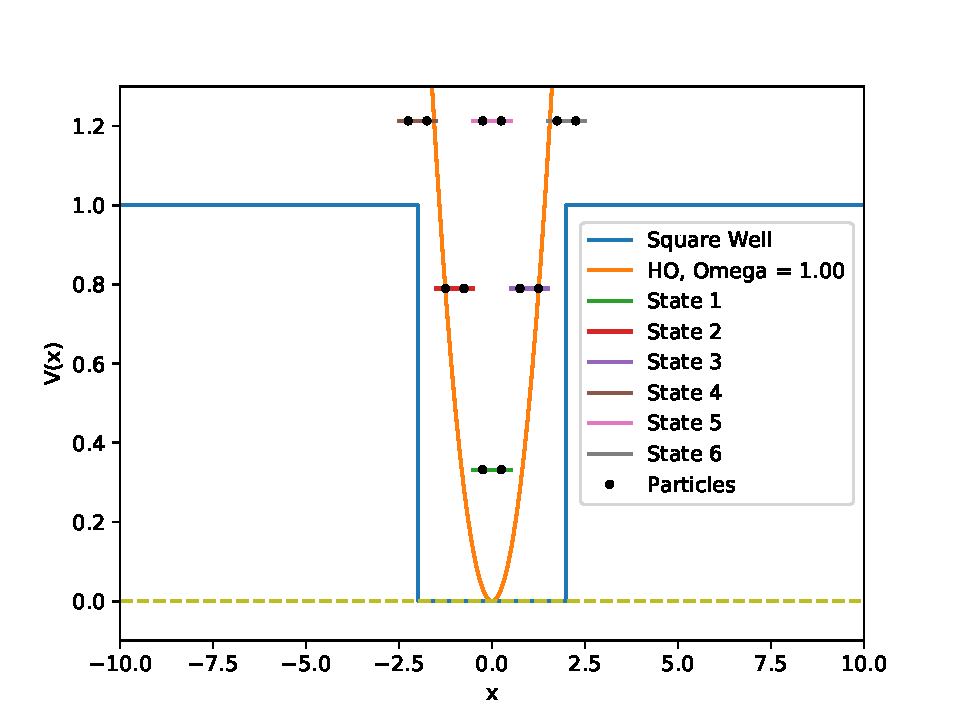
\includegraphics[width=\linewidth]{figures/SW_Energy_Levels}
\caption{The figure shows that the lowest three particle states for our specific finite square well potential in two dimensions are bound states, while the higher states are unbound. If only the bound states are occupied then harmonic oscillator basis functions are a reasonable fit to the potential, but not if unbound states are occupied.}
\label{fig: FSW_energy_levels}
\end{figure}

\section{Testing of the Diagonalization Program}

The testing of the VMC solver indirectly tests this program as well, and since the VMC tests for the single harmonic oscillator well were as good as they can be, we have focused on the double harmonic oscillator well and the finite square well when testing this program.

\subsection{Double Harmonic Oscillator Well}
There are several test we can use to validate the coefficients we have found. One thing we can check is that the $L_2$-norm is a small number:
\begin{equation}
    ||\psi_{n^\prime}^\textrm{diag}-\psi_{n^\prime}^\textrm{exp}||_2 = \sqrt{\sum_i^N |\psi_{n^\prime}^\textrm{diag}(x_i)-\psi_{n^\prime}^\textrm{exp}(x_i)|^2} < \epsilon.
\end{equation}
Here $\psi_{n^\prime}^\textrm{diag}$ are the solutions (eigenvectors) we got from diagonalizing the single particle problem, while $\psi_{n^\prime}^\textrm{exp}$ are the approximations from the linear expansion in Eq.~(\ref{eq: Approximate SPWF2}). The $L_2$-norm being less than a small number $\epsilon$ would mean that the linear expansion approximations are reasonably similar to the solutions from diagonalizing. We can also do a similar test by plotting $\psi_{n^\prime}^\textrm{diag}$ and $\psi_{n^\prime}^\textrm{exp}$ together for various $n^\prime$ and checking that the two curves are (to some precision) on top of each other. We expect the result of both of these test to be best for low $n^\prime$ values and then get worse and worse as $n^\prime$ increases. We also expect that increasing the number of basis functions used in the linear expansion should improve the results and consequently give good results for a larger number of $n^\prime$.

\begin{table}[!ht]
  \centering
  \begin{tabular}{ | c | c | c | c | }
    \hline
    $n^\prime$ & Energy Levels & Basis Functions & $L_2$-norm\\*
    \hline
    $0$ & $20$ & $210$ & $0.246582153723$ %$0.2466$ 
    \\*
    \hline
    $0$ & $27$ & $378$ & $0.00288150262617$ %$0.0029$ 
    \\*
    \hline
    $9$ & $20$ & $210$ & $0.402442469552$ %$0.4024$ 
    \\*
    \hline
    $9$ & $27$ & $378$ & $0.175246533084$ %$0.1752$ 
    \\*
    \hline
  \end{tabular}
  \caption{$L2$-norm values for a double well potential in two dimensions with $\omega = 1$, $N = 1000$, $L_x = 4.0$ and $L_y = 0.0$. The basis functions column lists the number of basis functions used in the linear expansion. We see that for a given number of basis functions the $L2$-norm is better (smaller) for $n^\prime = 0$ than for $n^\prime = 9$, indicating that for larger $n^\prime$ we need a higher number of basis functions to get good results. We also see that for a given $n^\prime$, using more basis functions gives a better $L2$-norm.}
  \label{tab:L2-norm}
\end{table}

In Table \ref{tab:L2-norm} we have listed the $L2$-norm for $n^\prime = 0$ and $n^\prime = 9$ with $210$ and $378$ basis functions used for the linear expansion. The values in the table are for a double well potential in two dimensions. We see that the $L2$-norm is generally smaller when we are using more basis function as expected, and as $n^\prime$ increases we need more basis functions to get a good $L2$-norm. When using $378$ basis functions for the $n^\prime = 0$ case we get a reasonably good $L2$-norm, while for the other cases we should use more basis functions. We need one value of $n^\prime$ for every two particles in the system we want to study, so for a system with only two particles we only need $n^\prime = 0$, so $378$ basis functions should be sufficient. For a system with $20$ particles we would need $n^\prime = 0,1,\dots,9$, so based on the $L2$-norm for $n^\prime = 9$, using $378$ basis functions will probably not be enough for this system (in Table \ref{tab:DoubleHOTest2D} we used $630$ basis functions to get a good result for this system). 

In Figure \ref{fig:nPrime0} we see the plots of $\psi_{n^\prime}^\textrm{diag}$ and $\psi_{n^\prime}^\textrm{exp}$ together for $n^\prime = 0$. Again we have used a two dimensional double well potential. For Figure \ref{fig:nPrime0a} we used $210$ basis functions for $\psi_{n^\prime}^\textrm{exp}$. We see $\psi_{n^\prime}^\textrm{exp}$ has a somewhat similar shape as $\psi_{n^\prime}^\textrm{diag}$, but the error is significant close to $x = 0$. In Figure \ref{fig:nPrime0b} we have increased the number of basis functions to $378$, and as expected $\psi_{n^\prime}^\textrm{exp}$ matches $\psi_{n^\prime}^\textrm{diag}$ much better. Figure \ref{fig:nPrime9} is equivalent to Figure \ref{fig:nPrime0}, but for $n^\prime = 9$. Here as well we see that with $210$ basis functions we get significant errors, while with $378$ basis functions the match between $\psi_{n^\prime}^\textrm{exp}$ and $\psi_{n^\prime}^\textrm{diag}$ is much better. However, for $n^\prime = 9$, even with $378$ basis function we still do not get a great match. Just as for with the $L2$-norm, this shows that increasing the number of basis functions improves the results, and that greater $n^\prime$ values require a greater number of basis functions to yield good results.


\begin{figure}
    \centering
    \begin{subfigure}{0.5\textwidth}
        \centering
        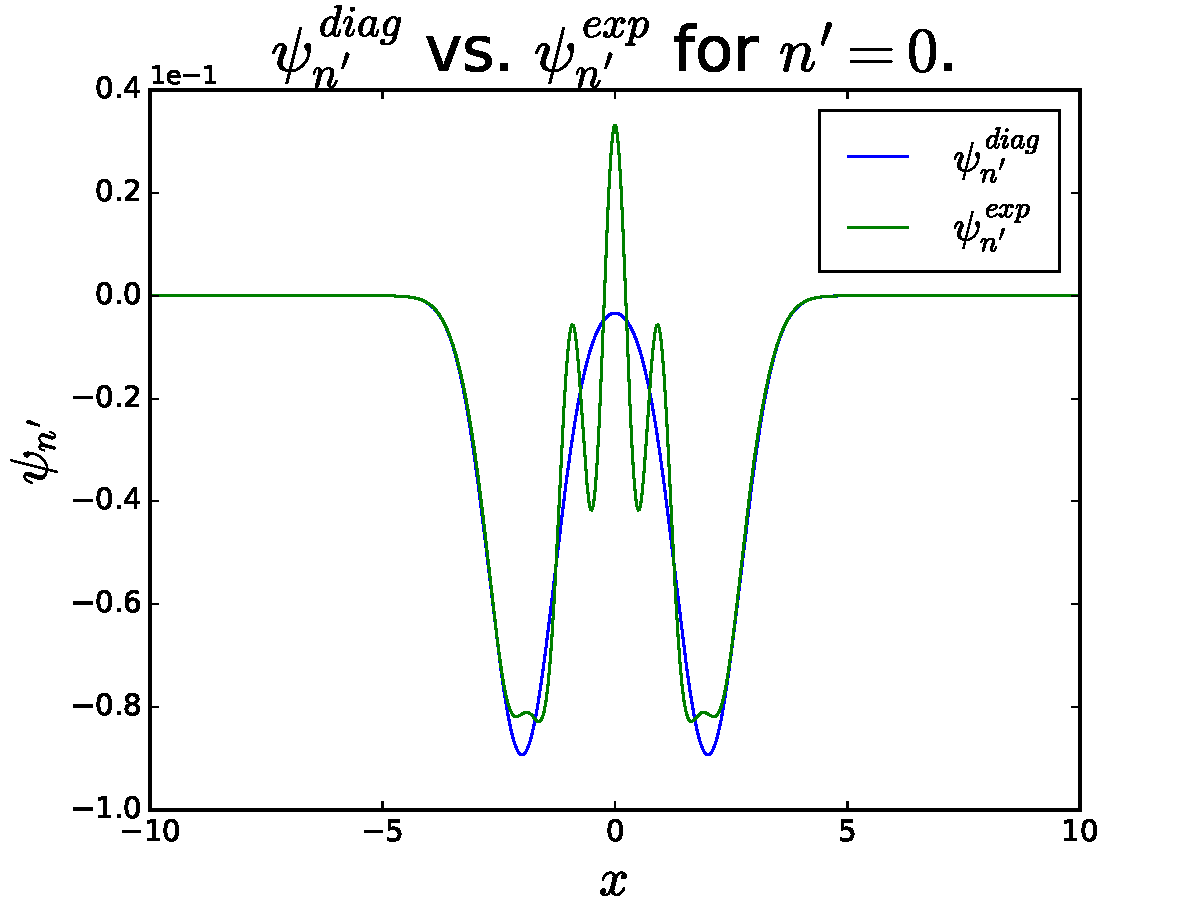
\includegraphics[scale=0.4]{figures/psiComp/psiComp_nPrime0_BF210}
        \caption{$210$ Basis Functions ($20$ Energy Levels).}
        \label{fig:nPrime0a}
    \end{subfigure}%
    ~ 
    \begin{subfigure}{0.5\textwidth}
        \centering
        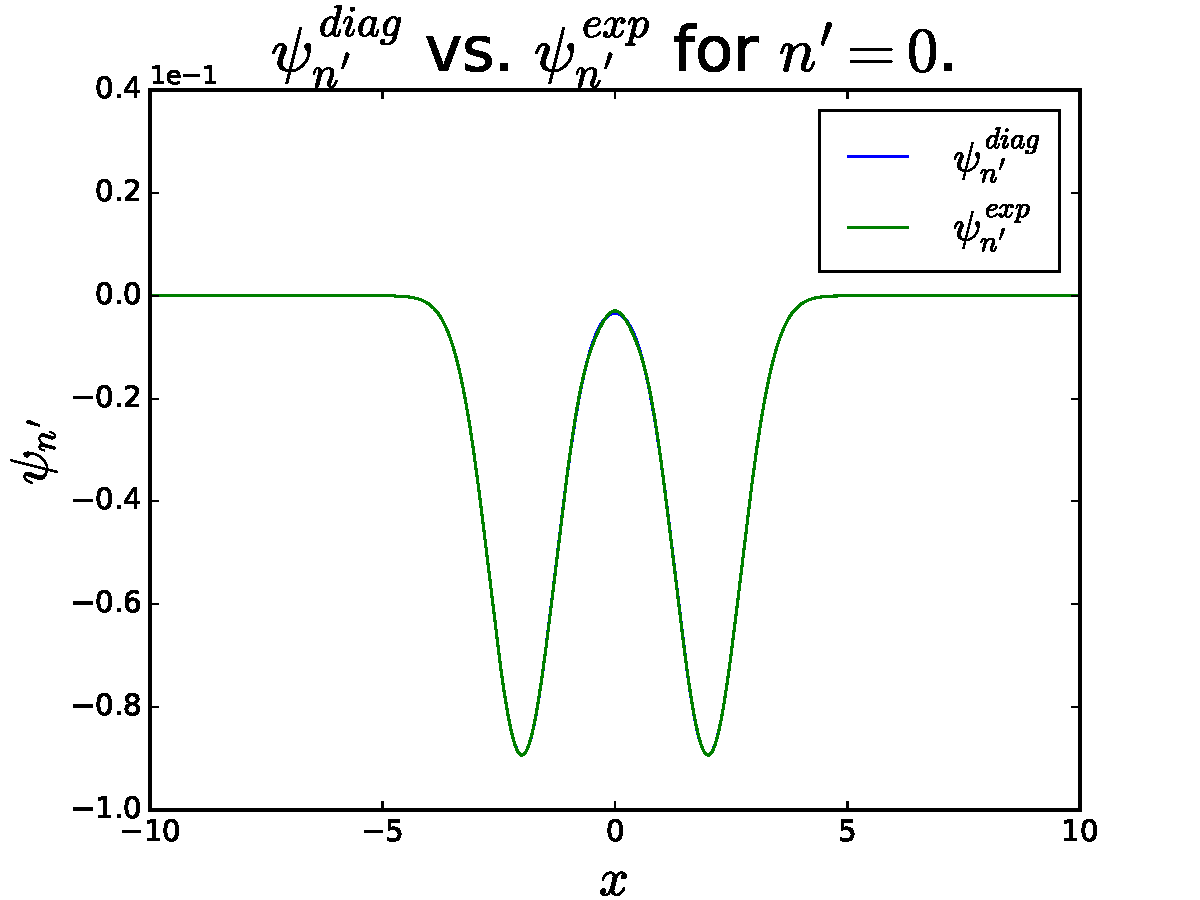
\includegraphics[scale=0.4]{figures/psiComp/psiComp_nPrime0_BF378}
        \caption{$378$ Basis Functions ($27$ Energy Levels).}
        \label{fig:nPrime0b}
    \end{subfigure}
    \caption{$\psi_{n^\prime}^\textrm{diag}$ vs. $\psi_{n^\prime}^\textrm{exp}$ for a two-dimensional double well potential with $n^\prime = 0$, $N=1000$, $L_x = 4.0$, $L_y = 0$ and $\omega = 1$. We see that when we use only $210$ basis functions the linear expansion approximation is a fairly bad match to the solution we got from diagonalizing. However, the shape is still somewhat similar. When we increase the number of basis functions to $378$ we get a pretty good match.}
    \label{fig:nPrime0}
\end{figure}

\begin{figure}
    \centering
    \begin{subfigure}{0.5\textwidth}
        \centering
        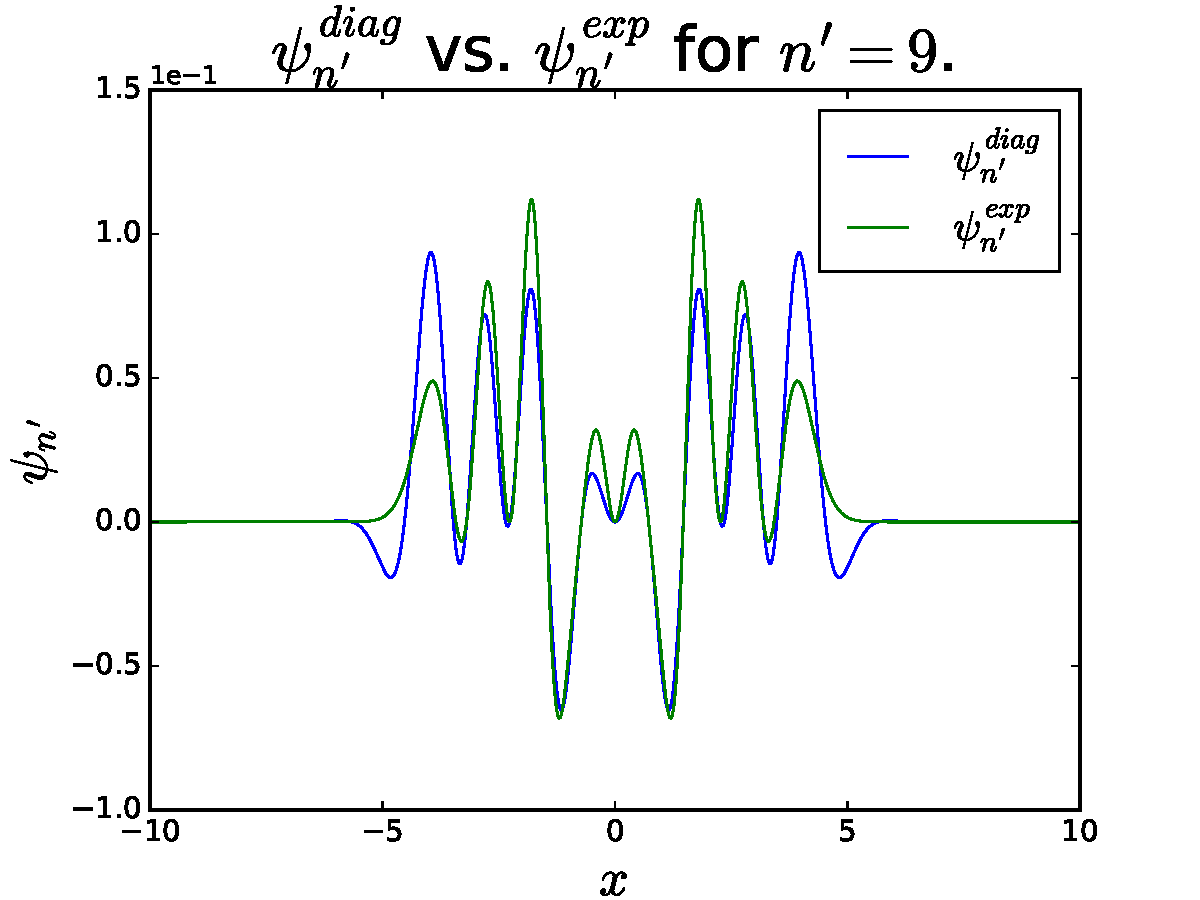
\includegraphics[scale=0.4]{figures/psiComp/psiComp_nPrime9_BF210}
        \caption{$210$ Basis Functions ($20$ Energy Levels).}
        \label{fig:nPrime9a}
    \end{subfigure}%
    ~ 
    \begin{subfigure}{0.5\textwidth}
        \centering
        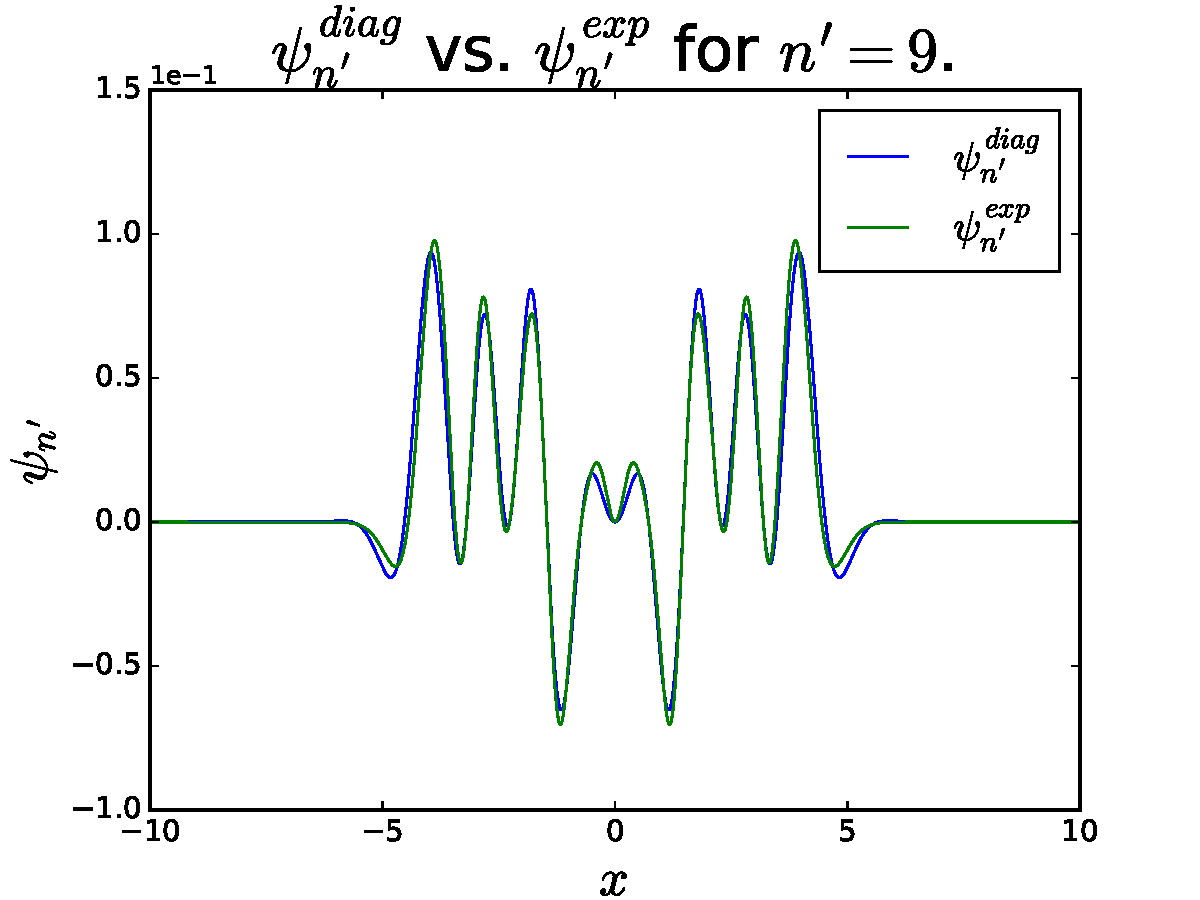
\includegraphics[scale=0.4]{figures/psiComp/psiComp_nPrime9_BF378}
        \caption{$378$ Basis Functions ($27$ Energy Levels).}
        \label{fig:nPrime9b}
    \end{subfigure}
    \caption{$\psi_{n^\prime}^\textrm{diag}$ vs. $\psi_{n^\prime}^\textrm{exp}$ for a two-dimensional double well potential with $n^\prime = 9$, $N=1000$, $L_x = 4.0$, $L_y = 0$ and $\omega = 1$. As for the $n^\prime = 0$ case we get a bad match when using only $210$ basis functions. Still, there are some similarities between the linear expansion approximation and the solution. When we increase the number of basis functions to $378$ we get a significantly better match, but it is not quite as good as in the $n^\prime = 0$ case.}
    \label{fig:nPrime9}
\end{figure}

Another test we can do is to check that the norm of $\psi^\textrm{exp}$ for each dimension separately is approximately equal to $1$ and that the accuracy increases with increasing number of basis function like in the previous tests. The norm is given by
\begin{equation}
    ||\psi|| = \sqrt{\langle \psi|\psi \rangle},
\end{equation}
and we want the following to be true
\begin{equation}
    ||\psi_{n^\prime}^\textrm{exp}(x)|| \approx ||\psi_{n^\prime}^\textrm{exp}(y)|| \approx ||\psi_{n^\prime}^\textrm{exp}(z)|| \approx 1,
\end{equation}
in the three dimensional case. For this test we will use the same system as for the two previous tests, i.e. a two dimensional system, where the potential is a double harmonic oscillator well in the $x$-dimension and a single harmonic oscillator well in the $y$-dimension. Table \ref{tab:NormE20} and Table \ref{tab:NormE27} lists $||\psi_{n^\prime}^\textrm{exp}(x)||$ and $||\psi_{n^\prime}^\textrm{exp}(y)||$ for $20$ energy levels and $27$ energy levels respectively. Note that since we here look at each dimension separately the number of energy levels and the number basis functions are the same. The tables list the results for $n^\prime = 0,1,\dots,9$. In both tables $||\psi_{n^\prime}^\textrm{exp}(y)||$ is exactly $1$ to machine precision for all $n^\prime$. This makes sense since the potential for the $y$-dimension is a single harmonic oscillator well and we use single harmonic oscillator functions as basis functions. For the $x$-dimension on the other hand we have a double well potential and should therefore expect some deviation from $1$. As with the previous tests we expect that the deviation should increase as we increase $n^\prime$. From Table \ref{tab:NormE20} we see that the deviation does not strictly increase with increasing $n^\prime$, but that significantly increasing $n^\prime$, significantly increases the deviation (e.g. going from $n^\prime = 0$ to $n^\prime = 9$). If we compare Table \ref{tab:NormE20} with Table \ref{tab:NormE27} we again see that increasing the number of basis functions improves the results for all $n^\prime$.

\begin{table}[!ht]
  \centering
  \begin{subtable}{.4\linewidth}
      \centering
      \begin{tabular}{ | c | c | c | }
        \hline
        $n^\prime$ & $||\psi_{n^\prime}^\textrm{exp}(x)||$ & $||\psi_{n^\prime}^\textrm{exp}(y)||$\\*
        \hline
        $0$ & $0.999816193222$ & $1.0$\\*
        \hline
        $1$ & $0.999930888372$ & $1.0$\\*
        \hline
        $2$ & $0.996501279797$ & $1.0$\\*
        \hline
        $3$ & $0.998471329039$ & $1.0$\\*
        \hline
        $4$ & $0.974110444039$ & $1.0$\\*
        \hline
        $5$ & $0.986589494196$ & $1.0$\\*
        \hline
        $6$ & $0.904585077720$ & $1.0$\\*
        \hline
        $7$ & $0.939665912097$ & $1.0$\\*
        \hline
        $8$ & $0.817567381049$ & $1.0$\\*
        \hline
        $9$ & $0.850878481823$ & $1.0$\\*
        \hline
      \end{tabular}
      \caption{$20$ Basis Functions ($20$ Energy Levels)}
      \label{tab:NormE20}
  \end{subtable}
  ~
  \begin{subtable}{.4\linewidth}
    \centering
    \begin{tabular}{ | c | c | c | }
        \hline
        $n^\prime$ & $||\psi_{n^\prime}^\textrm{exp}(x)||$ & $||\psi_{n^\prime}^\textrm{exp}(y)||$\\*
        \hline
        $0$ & $0.999999977026$ & $1.0$\\*
        \hline
        $1$ & $0.999999918994$ & $1.0$\\*
        \hline
        $2$ & $0.999998831156$ & $1.0$\\*
        \hline
        $3$ & $0.999996288163$ & $1.0$\\*
        \hline
        $4$ & $0.999974270670$ & $1.0$\\*
        \hline
        $5$ & $0.999926388426$ & $1.0$\\*
        \hline
        $6$ & $0.999675990997$ & $1.0$\\*
        \hline
        $7$ & $0.999175833447$ & $1.0$\\*
        \hline
        $8$ & $0.997471707200$ & $1.0$\\*
        \hline
        $9$ & $0.994189907404$ & $1.0$\\*
        \hline
    \end{tabular}
    \caption{$27$ Basis Functions ($27$ Energy Levels)}
    \label{tab:NormE27}
  \end{subtable}
  \caption{$||\psi_{n^\prime}^\textrm{exp}(x)||$ and $||\psi_{n^\prime}^\textrm{exp}(y)||$ values for a two-dimensional double well potential with $\omega = 1$, $N = 1000$, $L_x = 4.0$ and $L_y = 0.0$. Since we are looking at each dimension separately the number of basis functions is the same as the number of energy levels. In both tables $||\psi_{n^\prime}^\textrm{exp}(y)||$ is equal to $1$ to machine precision, while $||\psi_{n^\prime}^\textrm{exp}(x)||$ has some deviation from $1$. This is due to the double well being in the $x$-dimension, while the potential in the $y$-dimension is a single harmonic oscillator well. Since the basis functions we use are single harmonic oscillator functions, the results for the $y$-dimension should be exact. For $||\psi_{n^\prime}^\textrm{exp}(x)||$ we also see that the deviation from $1$ is smaller when we have more basis functions and that the deviation typically increases when $n^\prime$ increases (but not always).}
  \label{tab:Norm}
\end{table}

\subsection{Finite Square Well}
We now redo the above test, but for a finite square well potential instead of a double harmonic oscillator well potential. With the distance between the well center and each wall being $2$ and $V_0 = 1$, we get the results for the $L2$'norm listed in Table \ref{tab:L2-norm Square}. From the table we see that the $L2$'norm is better for $n^\prime = 0$ and worse for $n^\prime = 9$ than when we used a double well potential (Table \ref{tab:L2-norm}). The $L2$-norm for $n^\prime = 0$ is really good for both $210$ and $378$ basis functions, while for $n^\prime = 9$ it is not quite as good.
\begin{table}[!ht]
  \centering
  \begin{tabular}{ | c | c | c | c | }
    \hline
    $n^\prime$ & Energy Levels & Basis Functions & $L_2$-norm\\*
    \hline
    $0$ & $20$ & $210$ & $0.00253244921988$
    \\*
    \hline
    $0$ & $27$ & $378$ & $0.00119302677155$
    \\*
    \hline
    $9$ & $20$ & $210$ & $0.91578729592$
    \\*
    \hline
    $9$ & $27$ & $378$ & $0.75248968038$
    \\*
    \hline
  \end{tabular}
  \caption{$L2$-norm values for a finite square well potential in two dimensions with $\omega = 1$, $N = 1000$, $V_0 = 1$ and the distance between the center and each wall is $2$. The basis functions column lists the number of basis functions used in the linear expansion. For $n^\prime = 0$ the $L2$-norm is better than it was for the double well, but for $n^\prime = 9$ it is worse.}
  \label{tab:L2-norm Square}
\end{table}

When looking at Figure \ref{fig:nPrime0Square} and \ref{fig:nPrime9Square}, we see the same situation. $\psi_{n^\prime}^\textrm{exp}$ matches $\psi_{n^\prime}^\textrm{diag}$ really well for $n^\prime = 0$ even for $210$ basis functions, but for $n^\prime = 9$, even with $378$ basis functions, $\psi_{n^\prime}^\textrm{exp}$ is a bad approximation to $\psi_{n^\prime}^\textrm{diag}$.

\begin{figure}
    \centering
    \begin{subfigure}{0.5\textwidth}
        \centering
        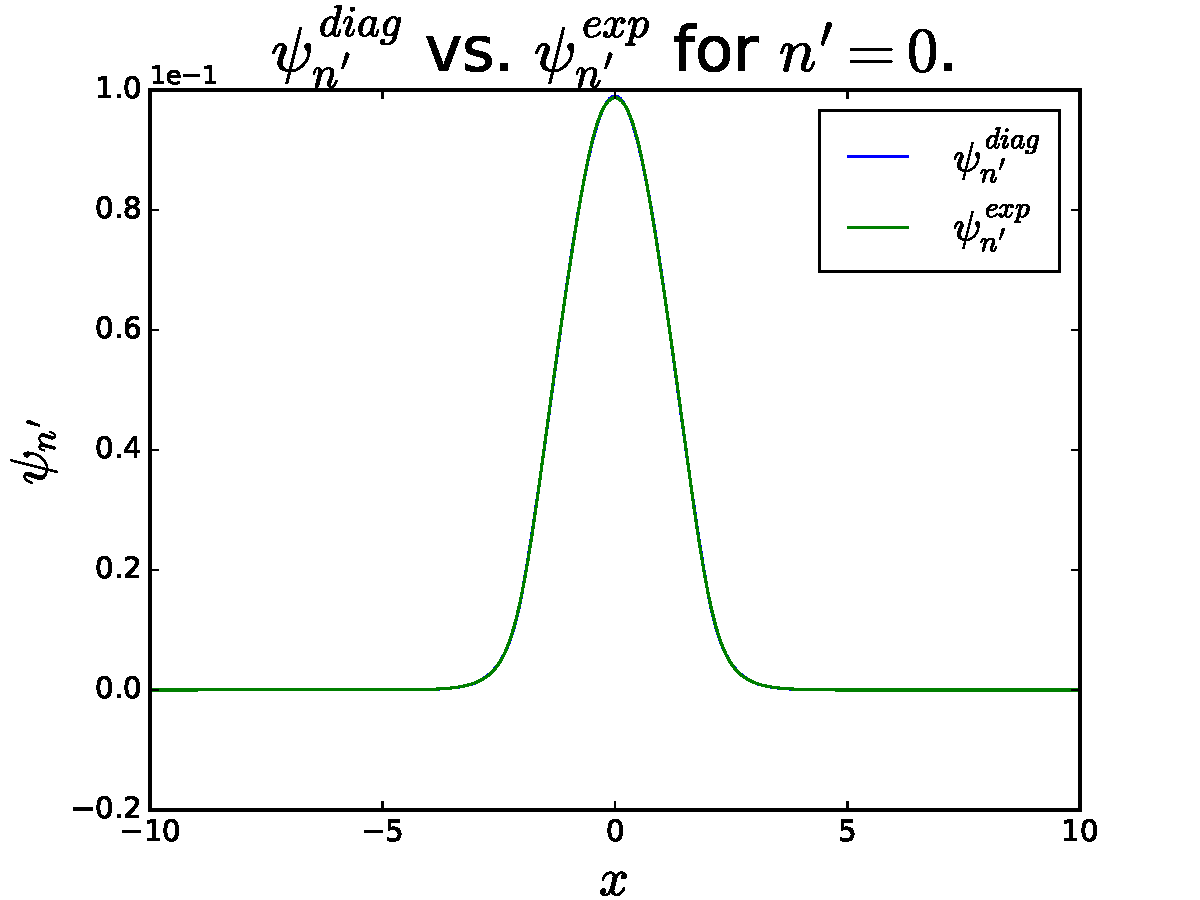
\includegraphics[scale=0.4]{figures/psiComp/psiCompSquare_nPrime0_BF210}
        \caption{$210$ Basis Functions ($20$ Energy Levels).}
        \label{fig:nPrime0aSquare}
    \end{subfigure}%
    ~ 
    \begin{subfigure}{0.5\textwidth}
        \centering
        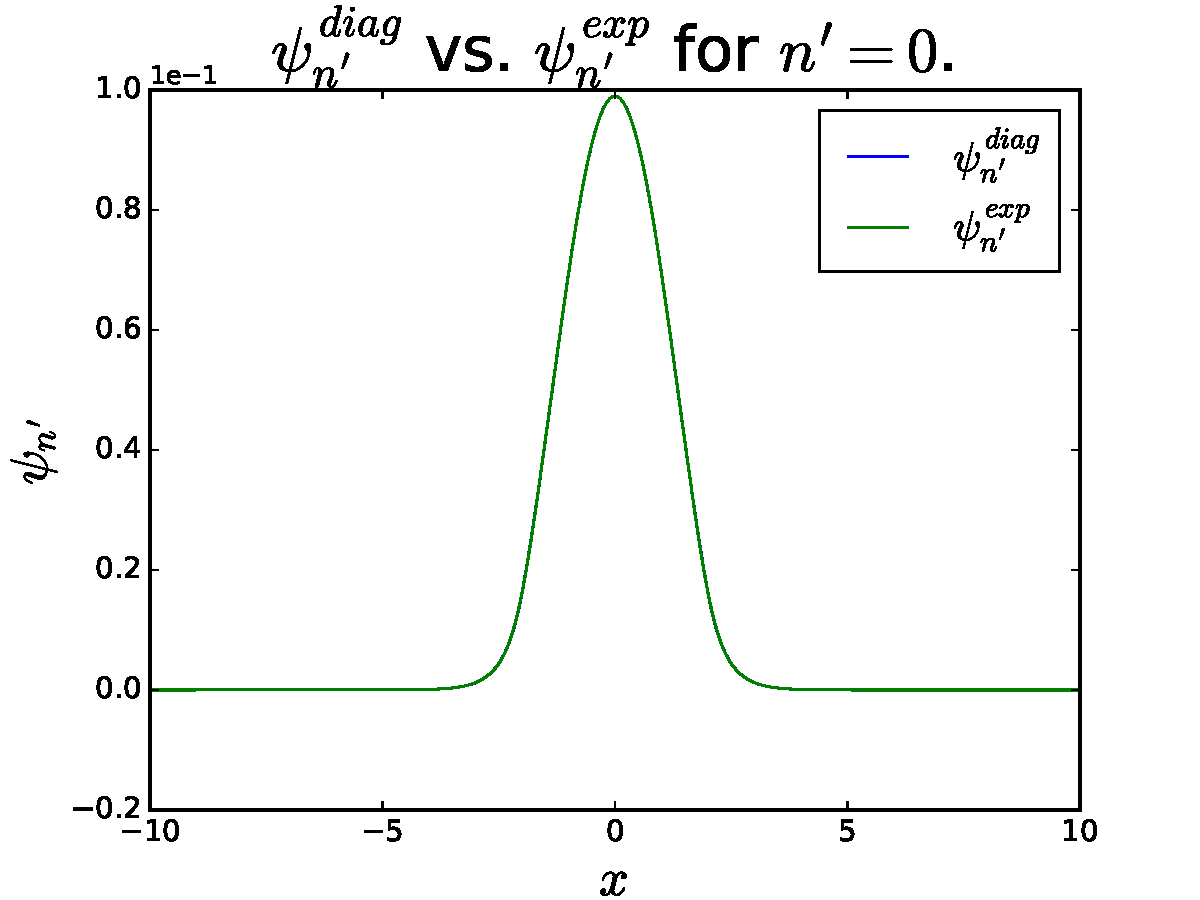
\includegraphics[scale=0.4]{figures/psiComp/psiCompSquare_nPrime0_BF378}
        \caption{$378$ Basis Functions ($27$ Energy Levels).}
        \label{fig:nPrime0bSquare}
    \end{subfigure}
    \caption{$\psi_{n^\prime}^\textrm{diag}$ vs. $\psi_{n^\prime}^\textrm{exp}$ for a two-dimensional finite square well potential with $n^\prime = 0$, $N=1000$, $\omega = 1$, $V_0 = 1$ and the distance between the center and each wall is $2$. We see that the curves are indistinguishable with both $210$ and $378$ basis functions.}
    \label{fig:nPrime0Square}
\end{figure}

\begin{figure}
    \centering
    \begin{subfigure}{0.5\textwidth}
        \centering
        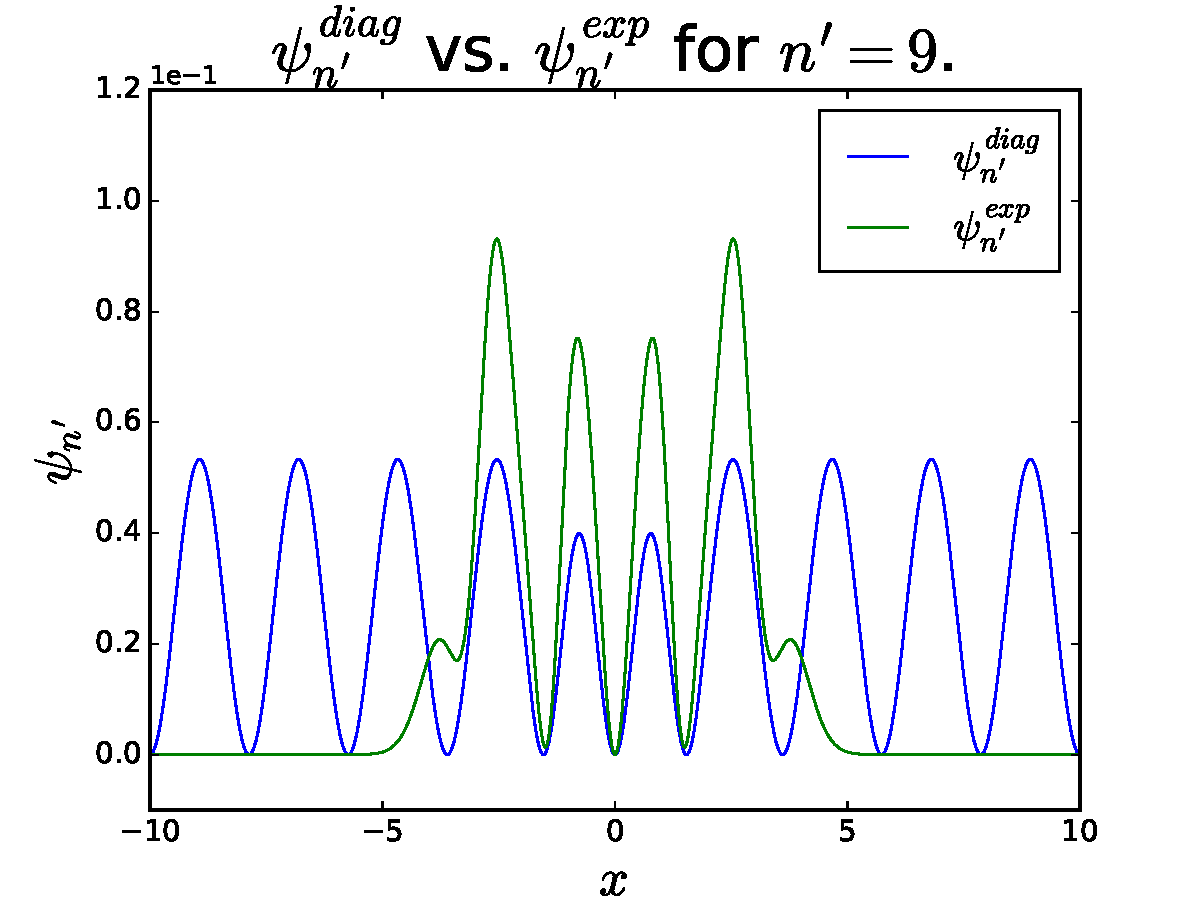
\includegraphics[scale=0.4]{figures/psiComp/psiCompSquare_nPrime9_BF210}
        \caption{$210$ Basis Functions ($20$ Energy Levels).}
        \label{fig:nPrime9aSquare}
    \end{subfigure}%
    ~ 
    \begin{subfigure}{0.5\textwidth}
        \centering
        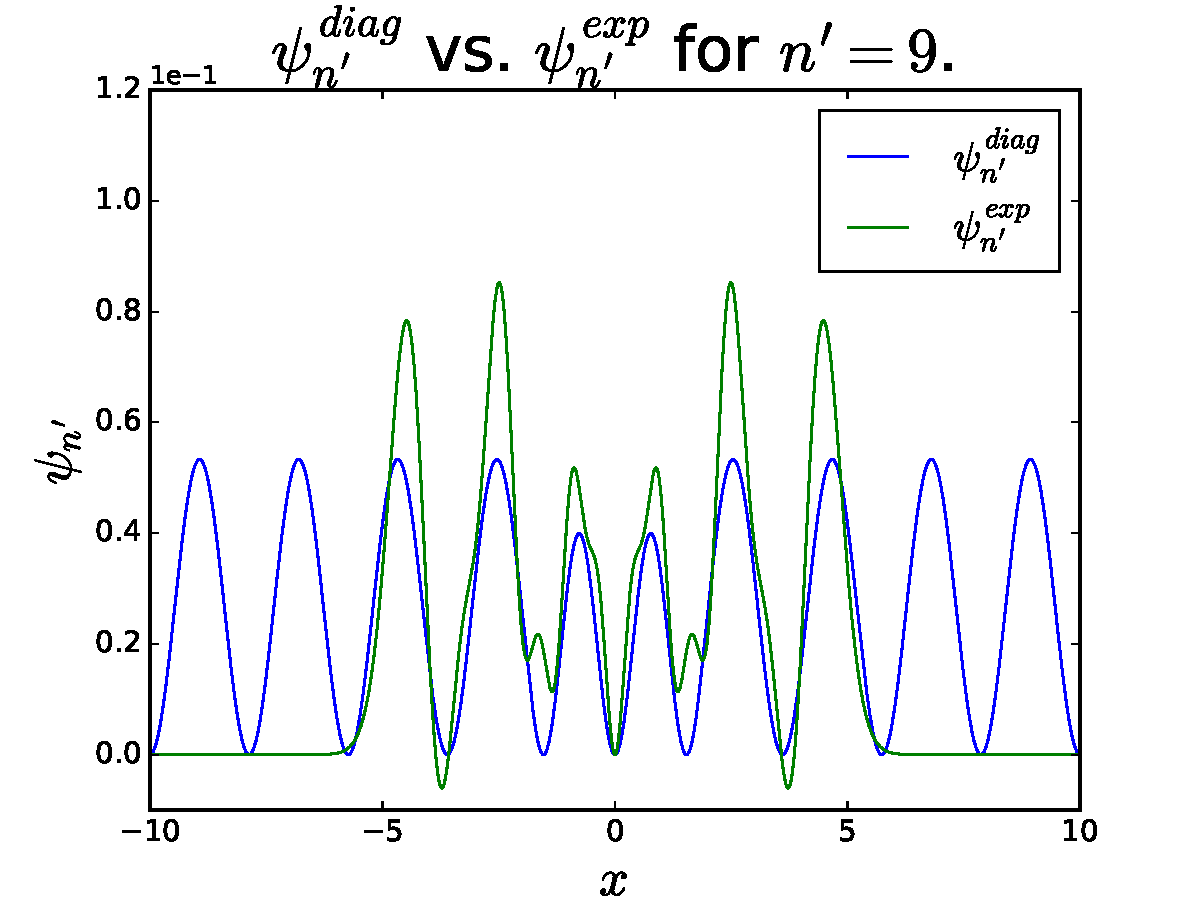
\includegraphics[scale=0.4]{figures/psiComp/psiCompSquare_nPrime9_BF378}
        \caption{$378$ Basis Functions ($27$ Energy Levels).}
        \label{fig:nPrime9bSquare}
    \end{subfigure}
    \caption{$\psi_{n^\prime}^\textrm{diag}$ vs. $\psi_{n^\prime}^\textrm{exp}$ for a two-dimensional finite square well potential with $n^\prime = 0$, $N=1000$, $\omega = 1$, $V_0 = 1$ and the distance between the center and each wall is $2$. We see that there is quite a big difference between the curves, but this is somewhat improved when increasing the number of basis functions from $210$ to $378$.}
    \label{fig:nPrime9Square}
\end{figure}

The results for the norm $||\psi_{n^\prime}^\textrm{exp}||$ are listed in Table \ref{tab:NormE20Square} and \ref{tab:NormE27Square}. Here we see that for $210$ basis functions the results are better for low $n^\prime$ than they were with a double well potential, but they also fall off much quicker as $n^\prime$ increases. We see that specifically we get good results for the first two $n^\prime$, which fits with what we saw about bound and unbound states in Section \ref{sec: FSW_vmc_test}. Here we look at each dimension separately and in 1D two states are bound and the rest are unbound. Thus $n^\prime = 0,1$ correspond to bound states while $n^\prime = 2,\dots,9$ correspond to unbound states. When increasing the number of basis functions from $210$ to $378$ the norms for all $n^\prime$ get closer to the target value $1$. However, for $378$ basis functions the results are worse than they were with a double well potential for all $n^\prime$.
\begin{table}[!ht]
  \centering
  \begin{subtable}{.4\linewidth}
      \centering
      \begin{tabular}{ | c | c | }
        \hline
        $n^\prime$ & $||\psi_{n^\prime}^\textrm{exp}(x)|| = ||\psi_{n^\prime}^\textrm{exp}(y)||$\\*
        \hline
        $0$ & $0.999998242918$\\*
        \hline
        $1$ & $0.999951314496$\\*
        \hline
        $2$ & $0.867214266147$\\*
        \hline
        $3$ & $0.768857257126$\\*
        \hline
        $4$ & $0.740421802754$\\*
        \hline
        $5$ & $0.725041681081$\\*
        \hline
        $6$ & $0.798534488615$\\*
        \hline
        $7$ & $0.798512568557$\\*
        \hline
        $8$ & $0.753433100459$\\*
        \hline
        $9$ & $0.757833831802$\\*
        \hline
      \end{tabular}
      \caption{$20$ Basis Functions ($20$ Energy Levels)}
      \label{tab:NormE20Square}
  \end{subtable}
  ~
  \begin{subtable}{.4\linewidth}
    \centering
    \begin{tabular}{ | c | c | c | }
        \hline
        $n^\prime$ & $||\psi_{n^\prime}^\textrm{exp}(x)|| = ||\psi_{n^\prime}^\textrm{exp}(y)||$\\*
        \hline
        $0$ & $0.9999991691$\\*
        \hline
        $1$ & $0.999986541$\\*
        \hline
        $2$ & $0.952180366269$\\*
        \hline
        $3$ & $0.887886200997$\\*
        \hline
        $4$ & $0.86139126026$\\*
        \hline
        $5$ & $0.779018497771$\\*
        \hline
        $6$ & $0.815843172148$\\*
        \hline
        $7$ & $0.829833024963$\\*
        \hline
        $8$ & $0.84973902467$\\*
        \hline
        $9$ & $0.859054357563$\\*
        \hline
    \end{tabular}
    \caption{$27$ Basis Functions ($27$ Energy Levels)}
    \label{tab:NormE27Square}
  \end{subtable}
  \caption{$||\psi_{n^\prime}^\textrm{exp}(x)||$ and $||\psi_{n^\prime}^\textrm{exp}(y)||$ values for a two-dimensional finite square well potential with $n^\prime = 0$, $N=1000$, $\omega = 1$, $V_0 = 1$ and the distance between the center and each wall is $2$. Since we are looking at each dimension separately the number of basis functions is the same as the number of energy levels. Unlike for the double well, here $||\psi_{n^\prime}^\textrm{exp}(x)||$ and $||\psi_{n^\prime}^\textrm{exp}(y)||$ are equal since the potential looks the same in both dimensions. Since the basis functions we use are single harmonic oscillator functions, and the potential is a finite square well, the norms are not exactly equal to the target value $1$. Just as for the double well potential, we see that the deviation from $1$ is smaller when we have more basis functions and that the deviation typically increases when $n^\prime$ increases (but not always).}
  \label{tab:NormSquare}
\end{table}

We redo the tests once more with a huge number of basis functions ($5050$), to see if we can get good results for $n^\prime = 9$. From Table \ref{tab:L2-norm Square100} we see that the $L2$-norm for $n^\prime = 0$ has improved even further, but now the $L2$-norm for $n^\prime = 9$ has also reached a reasonably good level. From Figure \ref{fig:nPrime0Square100} we see the same thing. For $n^\prime = 0$ the curves in Figure \ref{fig:nPrime0aSquare100} are still indistinguishable, like they were when using $210$ and $378$ basis functions. However, now for $n^\prime = 9$ as well, the curves in Figure \ref{fig:nPrime9bSquare100} are also nearly indistinguishable. There is only a slight visible difference on the left-most and right-most maxima. Also the results from Table \ref{tab:NormSquare100} confirms that $\psi_{n^\prime}^\textrm{exp}$ is a good approximation to $\psi_{n^\prime}^\textrm{diag}$ for $n^\prime = 9$ when we are using $5050$ basis functions. From the table we see that now the norm is really close to $1$ for all $n^\prime = 0,1,\dots,9$. 

\begin{table}[!ht]
  \centering
  \begin{tabular}{ | c | c | c | c | }
    \hline
    $n^\prime$ & Energy Levels & Basis Functions & $L_2$-norm\\*
    \hline
    $0$ & $100$ & $5050$ & $0.000265421396605$
    \\*
    \hline
    $9$ & $100$ & $5050$ & $0.0281926267177$
    \\*
    \hline
  \end{tabular}
  \caption{$L2$-norm values for a finite square well potential in two dimensions with $\omega = 1$, $N = 1000$, $V_0 = 1$ and the distance between the center and each wall is $2$. The basis functions column lists the number of basis functions used in the linear expansion. The $L2$-norm for $n^\prime = 0$ continues to be really good, but now the $L2$-norm for $n^\prime = 9$ has also reached a reasonably good level.}
  \label{tab:L2-norm Square100}
\end{table}



\begin{figure}
    \centering
    \begin{subfigure}{0.5\textwidth}
        \centering
        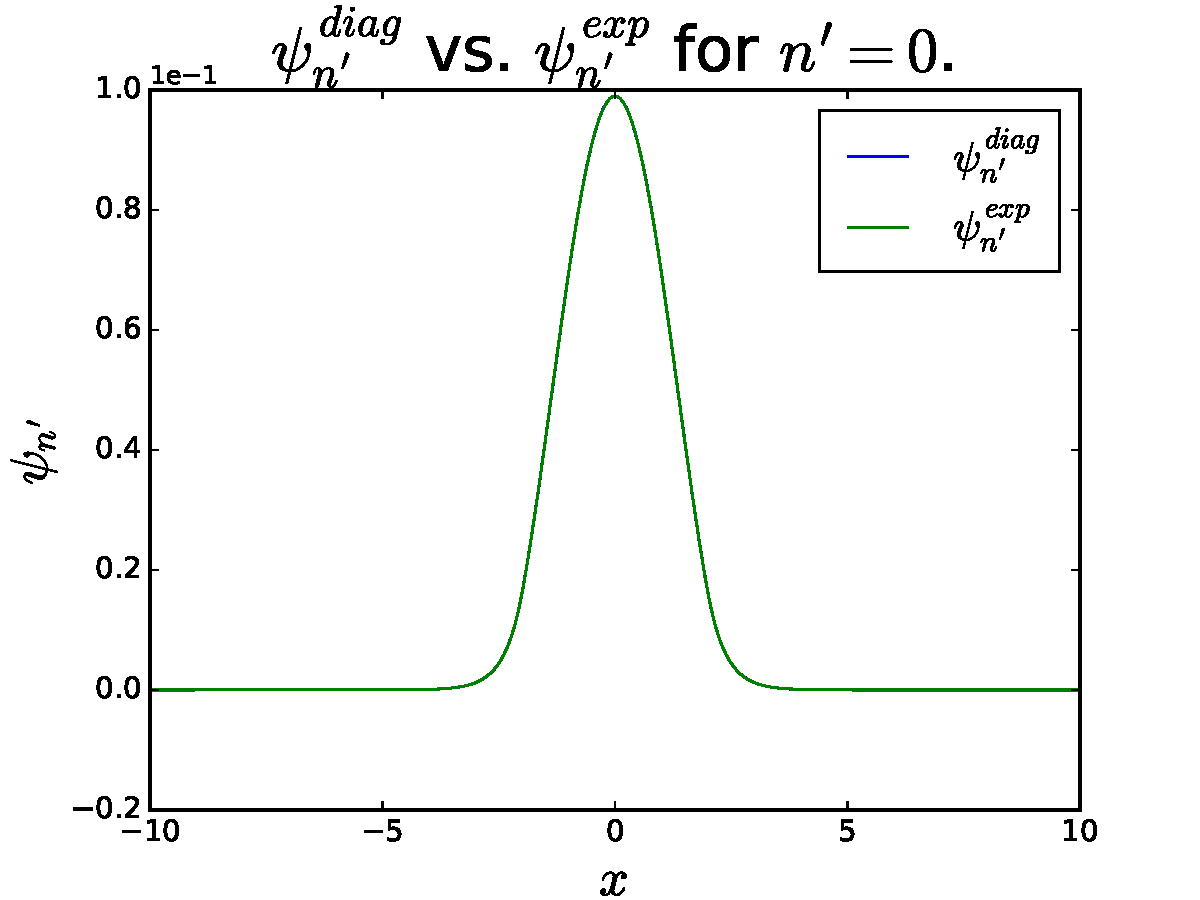
\includegraphics[scale=0.4]{figures/psiComp/psiCompSquare_nPrime0_BF5050}
        \caption{$5050$ Basis Functions ($100$ Energy Levels).}
        \label{fig:nPrime0aSquare100}
    \end{subfigure}%
    ~ 
    \begin{subfigure}{0.5\textwidth}
        \centering
        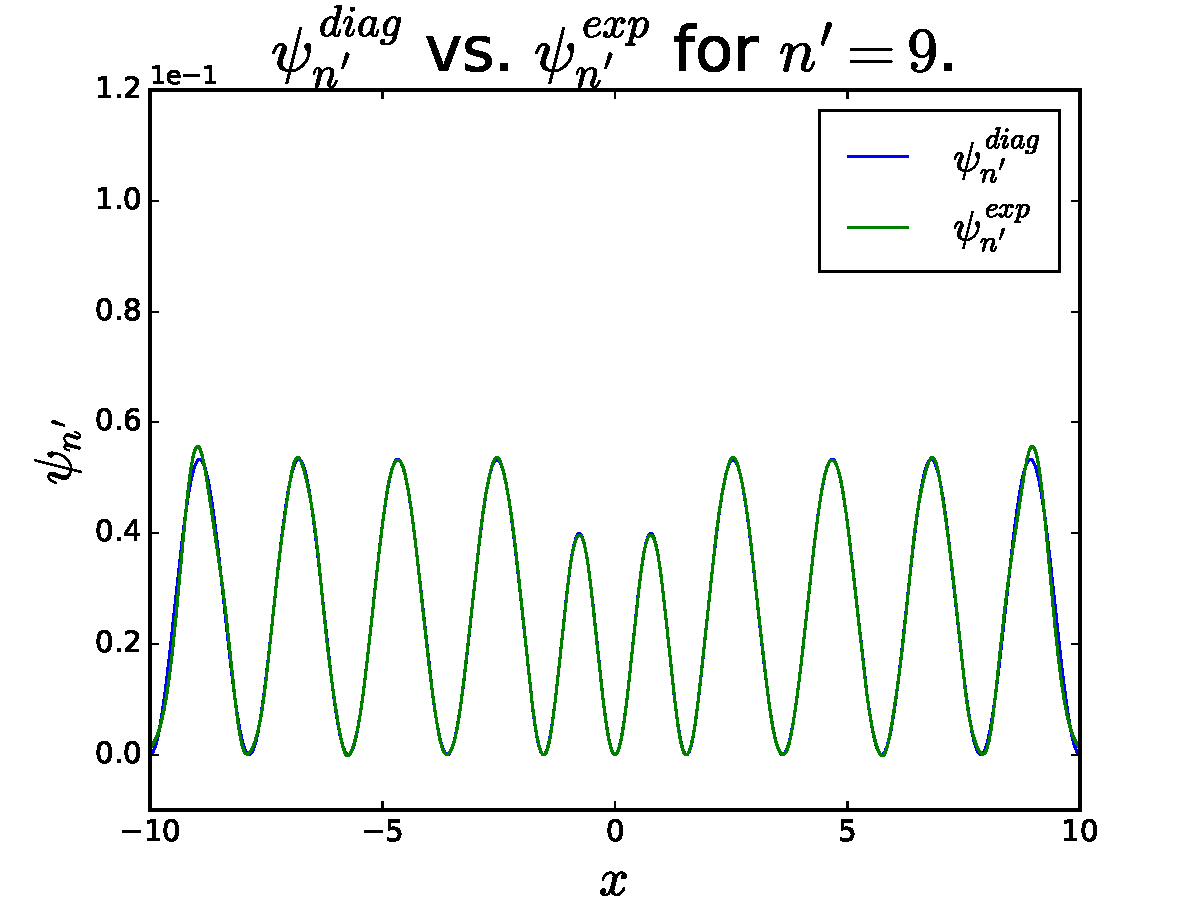
\includegraphics[scale=0.4]{figures/psiComp/psiCompSquare_nPrime9_BF5050}
        \caption{$5050$ Basis Functions ($100$ Energy Levels).}
        \label{fig:nPrime9bSquare100}
    \end{subfigure}
    \caption{$\psi_{n^\prime}^\textrm{diag}$ vs. $\psi_{n^\prime}^\textrm{exp}$ for a two-dimensional finite square well potential with $N=1000$, $\omega = 1$, $V_0 = 1$ and the distance between the center and each wall is $2$. We see that when using $5050$ basis functions, not only for $n^\prime = 0$, but also for $n^\prime = 9$ we have a really good match between the curves of $\psi_{n^\prime}^\textrm{diag}$ and $\psi_{n^\prime}^\textrm{exp}$. For $n^\prime = 9$ the match is vastly better than when using $210$ and $378$ basis functions.}
    \label{fig:nPrime0Square100}
\end{figure}


\begin{table}[!ht]
    \centering
    \begin{tabular}{ | c | c | c | }
        \hline
        $n^\prime$ & $||\psi_{n^\prime}^\textrm{exp}(x)|| = ||\psi_{n^\prime}^\textrm{exp}(y)||$\\*
        \hline
        $0$ & $0.999999972833$\\*
        \hline
        $1$ & $0.999999902664$\\*
        \hline
        $2$ & $0.999998457484$\\*
        \hline
        $3$ & $0.999996892487$\\*
        \hline
        $4$ & $0.999993799793$\\*
        \hline
        $5$ & $0.999988771956$\\*
        \hline
        $6$ & $0.999984406264$\\*
        \hline
        $7$ & $0.999977312106$\\*
        \hline
        $8$ & $0.99996981249$\\*
        \hline
        $9$ & $0.999964256428$\\*
        \hline
    \end{tabular}
    \caption{$||\psi_{n^\prime}^\textrm{exp}(x)||$ and $||\psi_{n^\prime}^\textrm{exp}(y)||$ values for a two-dimensional finite square well potential with $n^\prime = 0$, $N=1000$, $\omega = 1$, $V_0 = 1$ and the distance between the center and each wall is $2$. The number of energy levels is $100$, and since we are looking at each dimension separately the number of basis functions is the same as the number of energy levels. Unlike for the double well, here $||\psi_{n^\prime}^\textrm{exp}(x)||$ and $||\psi_{n^\prime}^\textrm{exp}(y)||$ are equal since the potential looks the same in both dimensions. Since the basis functions we use are single harmonic oscillator functions, and the potential is a finite square well, the norms are not exactly equal to the target value $1$. Now that we have significantly increased the number of basis functions compared to Table \ref{tab:NormSquare}, we see that the norm is reasonably close to $1$ for all $n^\prime = 0,1,\dots,9$.}
    \label{tab:NormSquare100}
\end{table}

We have seen that the results for a square well are better than those for a double harmonic oscillator well when $n^\prime$ is small, but then much worse for large $n^\prime$. A possible explanation for this is that the harmonic oscillator basis functions are a good fit for the square well as long as the energy is small enough that the finite nature of the well is not significant. Higher $n^\prime$ corresponds to higher energy, and when the energy is high enough that we are above the finite well, the potential is simply a straight line. At this point the harmonic oscillator basis function are probably no longer a good fit, so we need a much greater amount of them to be able to properly approximate $\psi_{n^\prime}^\textrm{diag}$.

\chapter{Optimizing Performance}\label{sec: OptimizingPerformance}

A variational Monte Carlo (VMC) simulation can quickly become very time consuming as we increase the number of particles in our system. In order to maintain efficiency of computations as the number of particles increases, it is important to optimize the simulation. One fairly common trait of suboptimal code is recalculation of identical values. An expression giving a value which needs to be used multiple times, should only be calculated once and the resulting values stored for later use. Doing this for various expressions was a big part of optimizing the VMC simulation. Another important optimization of the VMC simulation is the use of polymorphism. Most of the polymorphism used was included in the code from the beginning, but some were added later when optimizing the finished code. The third major optimization used, was to make the simulation parallelized using Open MPI\cite{Open MPI}.

\section{Storing Reused Data}

Storing various values which are used several times, instead of recalculating them every time, saves a lot of CPU time. This is particularly true as the number of particles increases to large numbers. By storing the values in matrices, we can simply access the matrix element of the value we need when we need it, rather than recalculating it every time that value is needed. This section loosely follows Chapter 4.6 of Ref.~\cite{Jorgen}.

\subsection{Relative Distances}

The simplest reusable values to store for the VMC simulation are the relative distances between the positions of particles. Whenever a relative distance is needed, for example to calculate the Jastrow factor, we can access the corresponding matrix element instead of recalculating the distance. All the relative distances are calculated once when we initiate the simulation and stored in a symmetric matrix on the form
\begin{equation}
    \mathbf{r} = \mathbf{r}^T =
    \left( \begin{array}{ccccc} 0 & r_{12} & \dots & \dots & r_{1N}\\
                                r_{21} & 0 & \ddots &  & r_{2N}\\
                                \vdots & \ddots & \ddots & \ddots & \vdots\\
                                \vdots &  & \ddots & \ddots & r_{nN}\\
                                r_{N1} & r_{N2} & \dots & r_{Nn} & 0

             \end{array} \right),
\end{equation}
where $N$ is the number of particles and $n=N-1$. Naturally $r_{12} = r_{21}$ since both are the relative distance between particle $1$ and $2$, so the matrix is symmetric. This saves us some additional computation time when creating and updating the matrix since we only have to calculate the values in either the upper or lower triangular part of the matrix, and mirror the values onto the other triangular part. Since we only move one particle at a time in the simulation, we only need to update $N$ relative distances when a particle is moved, since moving particle $1$ does not change e.g. $r_{23}$. The relative distance matrix is updated by the "updateDistances" function whenever a particle is moved.

\lstset{language=c++}
\begin{lstlisting}[caption={Function for updating the relative distances between particles whenever a particle is moved. $i$ is the moved particle so only the matrix elements where one of the indices is $i$ are changed when particle $i$ moves. Since no particle has any distance to itself, we split the loop in two so that we can exclude the $j=i$ case without using an if-test. Since the matrix is symmetric, $r_{ij} = r_{ji}$, and thus we can halve the number of distance calculations.}]
void ManyElectronsCoefficients::updateDistances(int currentParticle) {
    // Function for updating the distances between particles.
    int i = currentParticle;
    std::vector<double> r_i = m_system->getParticles()[i]->getPosition();

    for (int j=0; j<i; j++) {
        std::vector<double> r_j = m_system->getParticles()[j]->getPosition();
        double r_ij = 0;

        for (int d = 0; d < m_numberOfDimensions; d++) {
            r_ij += (r_i[d]-r_j[d])*(r_i[d]-r_j[d]);
        }
        m_distances(i,j) = m_distances(j,i) = sqrt(r_ij);
    }

    for (int j=i+1; j<m_numberOfParticles; j++) {
        std::vector<double> r_j = m_system->getParticles()[j]->getPosition();
        double r_ij = 0;

        for (int d = 0; d < m_numberOfDimensions; d++) {
            r_ij += (r_i[d]-r_j[d])*(r_i[d]-r_j[d]);
        }
        m_distances(i,j) = m_distances(j,i) = sqrt(r_ij);
    }
    
}
\end{lstlisting}

\subsection{Slater Matrices}

The Slater matrices consists of single particle wave functions $\phi_j(\mathbf{r}_i)$, and these single particle wave functions are used repeatedly in the VMC simulations, to for example calculate  the Metropolis ratio, update the inverse Slater matrices, etc. However, a given single particle wave functions only changes when the corresponding particles position changes. Consequently we can avoid having to recalculate these single particle wave functions by storing them in a matrix, and update the relevant elements whenever a particle is moved, just as we did for the relative distances. Whenever we need a given single particle wave function, we then simply access the corresponding element of the matrix. In the code we have named this matrix "m\_SPWFmat", and it is a concatenation of the spin-up and spin-down Slater matrices
\begin{equation}
    \mathbf{S} = \textrm{join}(\mathbf{S}^\uparrow, \mathbf{S}^\downarrow) =
    \left( \begin{array}{cccc} \phi_1(\mathbf{r}_1) & \phi_1(\mathbf{r}_2) & \dots & \phi_1(\mathbf{r}_N)\\
                                \phi_2(\mathbf{r}_1) & \phi_2(\mathbf{r}_2) & \dots & \phi_2(\mathbf{r}_N)\\
                                \vdots & \vdots & \ddots & \vdots\\
                                \phi_{N/2}(\mathbf{r}_1) & \phi_{N/2}(\mathbf{r}_2) & \dots & \phi_{N/2}(\mathbf{r}_N)

             \end{array} \right),
\end{equation}
where $\textrm{join}(\mathbf{S}^\uparrow, \mathbf{S}^\downarrow)$ means that we are joining the columns of the spin-up Slater matrix $\mathbf{S}^\uparrow$ and the spin-down matrix $\mathbf{S}^\downarrow$.

Not only the single particle wave functions, but also their gradients and Laplacians are used repeatedly in the simulation. Therefore to optimize further we create corresponding matrices containing these gradients and Laplacians. In the code the gradient matrix is called "m\_SPWFDMat" and is on the form
\begin{equation}
    \left( \begin{array}{cccc} \nabla\phi_1(\mathbf{r}_1) & \nabla\phi_1(\mathbf{r}_2) & \dots & \nabla\phi_1(\mathbf{r}_N)\\
                                \nabla\phi_2(\mathbf{r}_1) & \nabla\phi_2(\mathbf{r}_2) & \dots & \nabla\phi_2(\mathbf{r}_N)\\
                                \vdots & \vdots & \ddots & \vdots\\
                                \nabla\phi_{N/2}(\mathbf{r}_1) & \nabla\phi_{N/2}(\mathbf{r}_2) & \dots & \nabla\phi_{N/2}(\mathbf{r}_N)

             \end{array} \right),
\end{equation}
while the Laplacian matrix is called "m\_SPWFDDMat" and is on the form
\begin{equation}
    \left( \begin{array}{cccc} \nabla^2\phi_1(\mathbf{r}_1) & \nabla^2\phi_1(\mathbf{r}_2) & \dots & \nabla^2\phi_1(\mathbf{r}_N)\\
                                \nabla^2\phi_2(\mathbf{r}_1) & \nabla^2\phi_2(\mathbf{r}_2) & \dots & \nabla^2\phi_2(\mathbf{r}_N)\\
                                \vdots & \vdots & \ddots & \vdots\\
                                \nabla^2\phi_{N/2}(\mathbf{r}_1) & \nabla^2\phi_{N/2}(\mathbf{r}_2) & \dots & \nabla^2\phi_{N/2}(\mathbf{r}_N)

             \end{array} \right).
\end{equation}

\subsection{Jastrow Matrices}

The Jastrow factor we are using for our simulations is on the form
\begin{equation}
    \prod_{i<j}^N \exp\left(\frac{ar_{ij}}{1+\beta r_{ij}}\right) = \exp\left(\sum_{i<j}^N \frac{ar_{ij}}{1+\beta r_{ij}}\right),
\end{equation}
where $r_{ij}$ are the relative distances we have already stored in a matrix. From this we see that the distances matrix already optimizes the calculation of the Jastrow factor. However, we can further optimize this calculation by storing the full fraction 
\begin{equation}
    \frac{ar_{ij}}{1+\beta r_{ij}}
\end{equation}
in its own matrix. Element $ij$ of this new matrix would then be the value we get from the fraction for $r_{ij}$, and so for every relative distance we have a corresponding fraction value. This saves us from having to compute all of those fraction every time the Jastrow factor needs to be computed. Similarly to the relative distances matrix, only the relevant elements need to be recalculated whenever a particle is moved. 

The gradient of the Jastrow factor with respect to a given particle is
\begin{equation}
    \frac{\nabla_k J}{J} = \sum_{j\neq k} \frac{\mathbf{r}_{kj}}{r_{kj}} \frac{a}{(1+\beta r_{kj})^2},
\end{equation}
and we define
\begin{equation}
    d\mathbf{J}_{kj} \equiv \frac{\mathbf{r}_{kj}}{r_{kj}} \frac{a}{(1+\beta r_{kj})^2},
\end{equation}
which is antisymmetric, i.e.
\begin{equation}
    d\mathbf{J}_{kj} = -d\mathbf{J}_{jk}.
\end{equation}
The fractions $d\mathbf{J}_{kj}$ are used both for calculating the Jastrow gradients and for the Jastrow Laplacian. Storing $d\mathbf{J}_{kj}$ for all pairs of particles can therefore save us from recalculating it over and over. The matrix used for storing these fractions is fairly similar to the relative distances matrix, but with an antisymmetry instead of a symmetry. It is on the form

\begin{equation}
    d\mathbf{J} \equiv 
    \left( \begin{array}{ccccc} 0 & d\mathbf{J}_{12} & d\mathbf{J}_{13} & \dots & d\mathbf{J}_{1N}\\
                                -d\mathbf{J}_{12} & 0 & d\mathbf{J}_{23} & \dots & d\mathbf{J}_{2N}\\
                                -d\mathbf{J}_{13} & -d\mathbf{J}_{23} & \ddots & \ddots & \vdots\\
                                \vdots & \vdots & \ddots & \ddots & d\mathbf{J}_{nN}\\
                                -d\mathbf{J}_{1N} & -d\mathbf{J}_{2N} & \dots & -d\mathbf{J}_{nN} & 0

             \end{array} \right),
\end{equation}
with 
\begin{equation}
    d\mathbf{J} = -d\mathbf{J}^T.
\end{equation}
When a particle is moved we only need to update the relevant elements, which amount to one row and one column. We also store the gradients with respect to the different particles together in a matrix, since these gradients are used multiple times in the simulation. This matrix has dimensionality $(N\times d)$, where $d$ is the number of dimensions. Updating the gradient with respect to a given particle can now be simplified to 
\begin{equation}\label{eq:GradientSum}
    \frac{\nabla_k J^\textrm{new}}{J^\textrm{new}} = \sum_{j\neq k} d\mathbf{J}_{kj}^\textrm{new}, 
\end{equation}
but we can also further optimize the updating process by utilizing the "old" versions of the matrices, i.e. the matrices as they were before the most recent particle move: 
\begin{equation}
    \frac{\nabla_k J^\textrm{old}}{J^\textrm{old}} = \sum_{j\neq k} d\mathbf{J}_{kj}^\textrm{old}.
\end{equation}
We know that moving a particle $p$ only changes one row and one column in $d\mathbf{J}$. This means that for a particle $k\neq p$ only one term, $d\mathbf{J}_{kp}$, in the gradient sum has changed due to the move 
\begin{equation}\label{eq:UpdateGradient}
\begin{split}
    \frac{\nabla_{k\neq p} J^\textrm{new}}{J^\textrm{new}} &= \sum_{j\neq k} d\mathbf{J}_{kj}^\textrm{new}\\
    &= \sum_{j\neq k,p} d\mathbf{J}_{kj}^\textrm{old} + d\mathbf{J}_{kp}^\textrm{new}\\
    &= \sum_{j\neq k,p} d\mathbf{J}_{kj}^\textrm{old} + d\mathbf{J}_{kp}^\textrm{old} - d\mathbf{J}_{kp}^\textrm{old} + d\mathbf{J}_{kp}^\textrm{new}\\
    &= \frac{\nabla_{k\neq p} J^\textrm{old}}{J^\textrm{old}} - d\mathbf{J}_{kp}^\textrm{old} + d\mathbf{J}_{kp}^\textrm{new},
\end{split}
\end{equation}
where we have used 
\begin{equation}
    \frac{\nabla_{k\neq p} J^\textrm{old}}{J^\textrm{old}} = \sum_{j\neq k,p} d\mathbf{J}_{kj}^\textrm{old} + d\mathbf{J}_{kp}^\textrm{old}.
\end{equation}
We see then from Eq.~(\ref{eq:UpdateGradient}) that the gradient with respect to a particle $k\neq p$ can be updated by simply subtracting $d\mathbf{J}_{kj}^\textrm{old}$ and adding $d\mathbf{J}_{kj}^\textrm{new}$. For $k=p$ we still need to calculate the full sum in Eq.~(\ref{eq:GradientSum}). The function for updating the Jastrow matrices is listed below.

\lstset{language=c++}
\begin{lstlisting}[caption={Function for updating the Jastrow related matrices whenever a particle is moved. $p$ is the moved particle so only the matrix elements where one of the indices is $p$ are changed in "m\_JastrowMat" and "m\_dJastrowMat" when particle $p$ moves. In "m\_JastrowGrad" all elements need to be changed, however for $i\neq p$ the updating is simple and efficient. Since no particle has any distance to itself, we split the loop in two so that we can exclude the $j=p$ case without using an if-test. "m\_JastrowMat" is symmetric and "m\_dJastrowMat" is antisymmetric so for these we can halve the number of calculations.}]
void ManyElectronsCoefficients::updateJastrow(int currentParticle) {

    int p = currentParticle;
    std::vector<double> r_p = m_system->getParticles()[p]->getPosition();
    double beta = m_parameters[1];
    m_dJastrowMatOld = m_dJastrowMat;

    for (int j=0; j<p; j++) {
        std::vector<double> r_j = m_system->getParticles()[j]->getPosition();
        double r_pj = m_distances(p,j);
        double denom = 1 + beta*r_pj;

        m_JastrowMat(p,j) = m_a(p,j)*r_pj / denom;
        m_JastrowMat(j,p) = m_JastrowMat(p,j);

        for (int d = 0; d < m_numberOfDimensions; d++) {
            m_dJastrowMat(p,j,d) = (r_p[d]-r_j[d])/r_pj * m_a(p, j)/(denom*denom);
            m_dJastrowMat(j,p,d) = -m_dJastrowMat(p,j,d);
        }
    }
    for (int j=p+1; j<m_numberOfParticles; j++) {
        std::vector<double> r_j = m_system->getParticles()[j]->getPosition();
        double r_pj = m_distances(p,j);
        double denom = 1 + beta*r_pj;

        m_JastrowMat(p,j) = m_a(p,j)*r_pj / denom;
        m_JastrowMat(j,p) = m_JastrowMat(p,j);

        for (int d = 0; d < m_numberOfDimensions; d++) {
            m_dJastrowMat(p,j,d) = (r_p[d]-r_j[d])/r_pj * m_a(p, j)/(denom*denom);
            m_dJastrowMat(j,p,d) = -m_dJastrowMat(p,j,d);
        }
    }

    m_JastrowGradOld = m_JastrowGrad;

    for (int d = 0; d < m_numberOfDimensions; d++) {
        m_JastrowGrad(p, d) = 0;

        for (int j=0; j<p; j++) {
            m_JastrowGrad(p, d) += m_dJastrowMat(p,j,d);
        }
        for (int j=p+1; j<m_numberOfParticles; j++) {
            m_JastrowGrad(p, d) += m_dJastrowMat(p,j,d);
        }
        for (int i=0; i<p; i++) {
            m_JastrowGrad(i, d) = m_JastrowGradOld(i,d) - m_dJastrowMatOld(i,p,d) + m_dJastrowMat(i,p,d);
        }
        for (int i=p+1; i<m_numberOfParticles; i++) {
            m_JastrowGrad(i, d) = m_JastrowGradOld(i,d) - m_dJastrowMatOld(i,p,d) + m_dJastrowMat(i,p,d);
        }
    }
}
\end{lstlisting}


\section{Optimizing Hermite Polynomial Calculation}\label{sec:Optimizing Hermite}

As discussed in Section \ref{sec:Hamiltonians}, there are several ways we can calculate the Hermite polynomials we need for the single particle wave functions. In this section we will look at how virtual functions and polymorphism can be used to optimize these calculations. We create a super class "HermitePolynomials", which has sub classes for the Hermite polynomials, their derivatives and their double derivatives. So if we implement the first $20$ polynomials, we get a total of $60$ sub classes. Each of these sub classes have a virtual function called "eval" which takes a one-dimensional position (e.g. $x$) as argument and calculates the value corresponding to the sub class. For example the "eval" function of sub class "HermitePolynomial\_0" will return the value of the first Hermite polynomial for the given argument $x$, while the "eval" function of the sub class "dell\_HermitePolynomial\_0" will instead return the derivative of the first polynomial. In the VMC simulation the quantum numbers $nx$, $ny$ and $nz$ decide which polynomial we want the value, derivative, or double derivative of. By using the aforementioned sub classes, we can represent the Hermite polynomials as "HermitePolynomials" objects, which each holds one "eval" function. These objects can then be loaded into an array "m\_hermitePolynomials" in such a way that the first element of the array is the "HermitePolynomials" object representing the first polynomial, and so on for the rest of the elements. The way to calculate the Hermite polynomial for an arbitrary quantum number $nx$ is then simply
\lstset{language=c++}
\begin{lstlisting}[caption={}]
double HP = m\_hermitePolynomials[nx]->eval(x);
\end{lstlisting}
Thus we can calculate a Hermite polynomial for a given $nx$ without any consideration for any other Hermite polynomial. If we used if-tests instead we would have to test $nx$ against all values from $0$ to $nx$, which could be a lot of if-tests depending on how many Hermite polynomial we need for the full simulation. If we used the recursive method we would have to go through all Hermite polynomials up to the $nx$'th one. With our method we can also create similar arrays for the derivatives and the double derivatives. The downside to using this method is that it involves implementing a lot of sub classes. In our code we have included $50$ Hermite polynomials, which means $150$ total sub classes. It then greatly helps to use automatic code generation through e.g. SymPy\cite{SymPy}. We can then generate the sub classes automatically and copy them into the VMC code. The use of a find/replace function in a text editor quickly solves any general issue from the code generation. 

One thing to note is that this method of calculating Hermite polynomials is not necessarily faster than the recursive method. Using the Hermite polynomial expressions explicitly, which the polymorphism method does, involves a lot of power expressions. The recursive method becomes slower more quickly as the number of Hermite polynomials increases than the polymorphism method does, however even for quite a large number of Hermite polynomials the recursive method is faster if the power expressions are not calculated optimally. With sub optimal calculation of power expressions the polymorphism method did not break even with the recursive method until around $50$ Hermite polynomials were used in a timing test with two particles. An example of how power expressions can be optimized is listed below.
\lstset{language=c++}
\begin{lstlisting}[caption={Two methods for calculating $x^8$. The first method uses $7$ FLOPS, while the second method uses only $3$ FLOPS.}]
x8 = x*x*x*x*x*x*x*x;

x2 = x*x;
x4 = x2*x2;
x8 = x4*x4;
\end{lstlisting}
The listing shows two methods of calculating $x^8$, with the second method using less than half as many FLOPS as the first method. In our VMC simulation where we need to calculate a lot of Hermite polynomials with large power expressions, this optimization can save a lot of FLOPS. Our automatically generated code for the Hermite polynomials uses the "pow" function for calculating power expression. This function normally does not optimize the calculation of power expressions, because the optimizations in some cases can result in round-off errors. We use the compiler flag "ffast-math" to apply optimizations to mathematical functions such as "pow". Mathematically the functions are the same after the optimizations, but they are not exactly the same in floating-point arithmetic. Therefore, using the flag "can result in incorrect output for programs that depend on an exact implementation of IEEE or ISO rules/specifications for math functions" \cite{gccDocs}. Since using the flag can produce errors, we need to make sure that our results are consistent with and without using the flag. With the optimizations from the flag the polymorphism method becomes a lot more efficient than the recursive method even for few Hermite polynomials, and the benefit becomes greater and greater as the number of Hermite polynomials used increases. This is perfect for our simulation, since the number of Hermite polynomials needed increases as the number of basis functions we use increases. As mentioned earlier, increasing the number of basis functions improves the results, so this optimization allows us to get good results for significantly lower computational cost.

\section{Parallelization}\label{sec:Parallel}

The final optimization to discuss is the parallelization of the VMC simulation. The entire simulation is parallelized with Open MPI by dividing the number of Monte Carlo (MC) cycles among multiple nodes (processors). Each node gets its own seed for generating the random initial state of the system, and then runs its own VMC simulation with a fraction of the total amount of Monte Carlo cycles. After the nodes have finished their individual simulations, the results are brought together and averaged. When running a VMC simulation in parallel the individual simulations of nodes are completely independent of each other. This makes parallelization of VMC simulations very efficient, because the nodes only need to communicate at the very start and the very end. thus we do not have to worry about race conditions\footnote{A "race condition" can be defined as "Anomalous behavior due to unexpected critical dependence on the relative timing of events".\cite{Wheeler}} and synchronization\cite{Blaise} in the middle of the simulation. The only mid-simulation communication between nodes is when we are varying the variational parameters in order to find optimal parameters. However, this is typically done with small simulations where optimization is less important. After the optimal parameters have been found, a simulation with more MC cycles is ran using those parameters, so then there is no mid-simulation communication. 

With parallelization we can run the simulation on several nodes on a single computer. Modern computers typically have 4 or 8 processors, which can give a good amount of speed-up. We can also run the simulation on a super computer cluster in order to utilize even more processors. In this thesis we have only used four processors on a single computer, and simulated relatively small systems in order to show that the parallelization works. However, to get the true benefit of parallelization, a super computer should be used to run larger scale simulations. 

Since we do not need any mid-simulation communication between the nodes, we can expect a scaling which is approximately linear, i.e. if we double the amount of nodes we halve the computation time. When doing VMC calculations in parallel we have to be careful not to use too many processors for a small amount of MC cycles. If we have too many processors the amount of MC cycles for each processor might be too low to give good results. In addition the amount of MC cycles could end up being a non-integer number, which would not make sense.

%We use parallelization of code and specific compiler options to optimize the performance of our program. To parallelize our program we use MPI, and we also optimize with the $O3$ compiler flag of the GNU C++ compiler. The $O3$ flag tells the compiler to make optimizations to the code where it is possible, in order to reduce computation time. By parallelizing our program, we make it possible to run the program on multiple processors at once. We can run the program on several processors on a single computer (typically 4 or 8 processors) to get some speedup. However, we can also run it on a super computer cluster in order to utilize even more processors (we will use up to 64 processors in this project) and decrease computation time substantially. If the program is parallelized well we should see a speed-up of about a factor 2 when doubling the amount of processors. In general, Variational Monte Carlo simulations are simple to parallelize, so we should expect to achieve that amount of speed-up when running the code in parallel. When doing VMC calculations in parallel we have to be careful not to use too many processors for a small amount of MC cycles. If we have too many processors the amount of MC cycles for each processor might be too low to give good results. In addition the amount of MC cycles could end up being a non-integer number, which would not make sense.

\end{document}